\documentclass[journal,onecolumn]{IEEEtran}

% ---------------------------------------------------------------
% Packages
% ---------------------------------------------------------------
\usepackage{cite}
\usepackage{amsmath,amssymb,amsfonts}
\usepackage{graphicx}
\usepackage{textcomp}
\usepackage{xcolor}
\usepackage{booktabs}
\usepackage{array}
\usepackage{url}
\usepackage{hyperref}
\usepackage{float}
\usepackage{placeins}

% Float placement. These govern how much of a page LaTeX may fill with floats.
% The earlier values (textfraction 0.07, topfraction 0.9) permitted pages that
% were almost entirely figures, which is what produced the figure-dump pages.
% textfraction is the key one: it is the minimum share of a page that must be
% body text before LaTeX is allowed to place a float there.
\renewcommand{\topfraction}{0.70}          % max share of a page top used by floats
\renewcommand{\bottomfraction}{0.45}
\renewcommand{\textfraction}{0.25}         % at least a quarter of the page must be text
\renewcommand{\floatpagefraction}{0.70}    % a float-only page must be 70% full to be allowed
\renewcommand{\dbltopfraction}{0.70}
\renewcommand{\dblfloatpagefraction}{0.70}
\setcounter{topnumber}{2}
\setcounter{bottomnumber}{1}
\setcounter{totalnumber}{3}
\setcounter{dbltopnumber}{1}                % at most one full-width float per page top

\graphicspath{{figures_supplementary/}}

% Number figures and tables as S1, S2, ... so they match the citations
% used in the main manuscript.
\renewcommand{\thefigure}{S\arabic{figure}}
\renewcommand{\thetable}{S\arabic{table}}

\setlength{\textfloatsep}{10pt plus 2pt minus 4pt}
\setlength{\floatsep}{8pt plus 2pt minus 2pt}
\setlength{\intextsep}{10pt plus 2pt minus 2pt}

% ---------------------------------------------------------------
\begin{document}

\title{Supplementary Material for\\
``Evaluating the Predictive Utility of Synthetic Liver Cirrhosis Data for IoMT: A Comparative Study of Adversarial and Variational Architectures with Consensus-Based Quality Filtering''}

\author{\IEEEauthorblockN{Michael~Udousoro\IEEEauthorrefmark{1},~Mohammad~Farhan~Khan\IEEEauthorrefmark{1},~Fakhreldin~Saeed\IEEEauthorrefmark{1},~and~M.~Mursaleen\IEEEauthorrefmark{2}}
\IEEEauthorblockA{\IEEEauthorrefmark{1}Department of Computing, School of Engineering, Computing and Design, University of Roehampton, London, United Kingdom}
\IEEEauthorblockA{\IEEEauthorrefmark{2}Department of Medical Research, China Medical University Hospital, China Medical University, Taichung, Taiwan}}

\maketitle

% ===============================================================
\section{Scope of This Document}

The main manuscript reports the headline results within a strict page budget, which means a good deal of supporting detail had to be left out. This document supplies that detail. It is organised so that each section can be read on its own. All sixteen figures are cited directly from the main paper as Fig.~S1 to Fig.~S16. The eight tables, numbered Table~S1 to Table~S8, contain material that does not appear in the main paper at all.

Three kinds of material appear here. The first is methodological detail that a reader would need in order to reimplement the pipeline exactly: full architecture and optimiser settings, the preprocessing decisions, and the seeding regime that makes the results reproducible. The second is the complete per-feature statistical output. The main paper quotes a handful of Kolmogorov-Smirnov statistics to illustrate a pattern; Tables~\ref{tab:ks} to~\ref{tab:cohens} give all of them, for every feature and every generative method, so that the pattern can be checked rather than taken on trust. The third is the set of sensitivity and ablation analyses that justify particular parameter choices, chiefly the consensus tolerance of 5.0 and the output-perturbation level of $\sigma = 0.7$.

Nothing in this document changes any conclusion in the main paper. Where a number appears in both, it is the same number, produced by the same seeded run.

% ===============================================================
\section{Extended Methodology}

Fig.~\ref{figS:pipeline} gives an overview of the end-to-end pipeline referenced throughout this document and the main paper.

\subsection{Dataset and Preprocessing}

The Mayo Clinic Primary Biliary Cirrhosis trial data contains 418 patient records across 20 columns. Patients 1 to 312 were enrolled in the randomised placebo-controlled trial of D-penicillamine; patients 313 to 418 form a later observational cohort who consented to have basic measurements recorded but who did not undergo the full laboratory panel. Each of those 106 records is missing between nine and ten laboratory values.

This matters for how the missingness is handled. Imputing nine or ten values per record would mean inventing the majority of each patient's biochemical profile, and doing so from a cohort measured under a different protocol. The imputed values would carry the statistical structure of the trial arm rather than of the observational arm, which is precisely the kind of systematic bias that would then propagate into the generative models. Complete-case analysis was therefore chosen, leaving 276 records. The cost is a reduction in sample size and a restriction of the analysis to the randomised population; the benefit is that every value used is a value that was actually measured.

The patient identifier column is discarded as it carries no clinical signal. The remaining 19 columns comprise 11 continuous laboratory measurements, five binary clinical indicators, two ordinal variables, and the binary survival outcome. Categorical encodings are given in Section~III of the main paper.

All features are scaled to $[0,1]$ with a MinMaxScaler fitted \emph{only} on the 193-patient training partition. Fitting the scaler on the full dataset before splitting would leak information about the test patients into the training pipeline, and would inflate every downstream result. The same fitted scaler is applied to the test partition and inverted after generation to return synthetic records to clinical units.
Fig.~\ref{figS:corrmatrix} shows the correlation structure of the cohort the generative models are asked to reproduce. Bilirubin sits at the centre of a cluster of correlated markers of hepatic function, and N\_Days runs against them, which is the structure any useful synthetic record must preserve.
\begin{figure}[!tb]
  \centering
  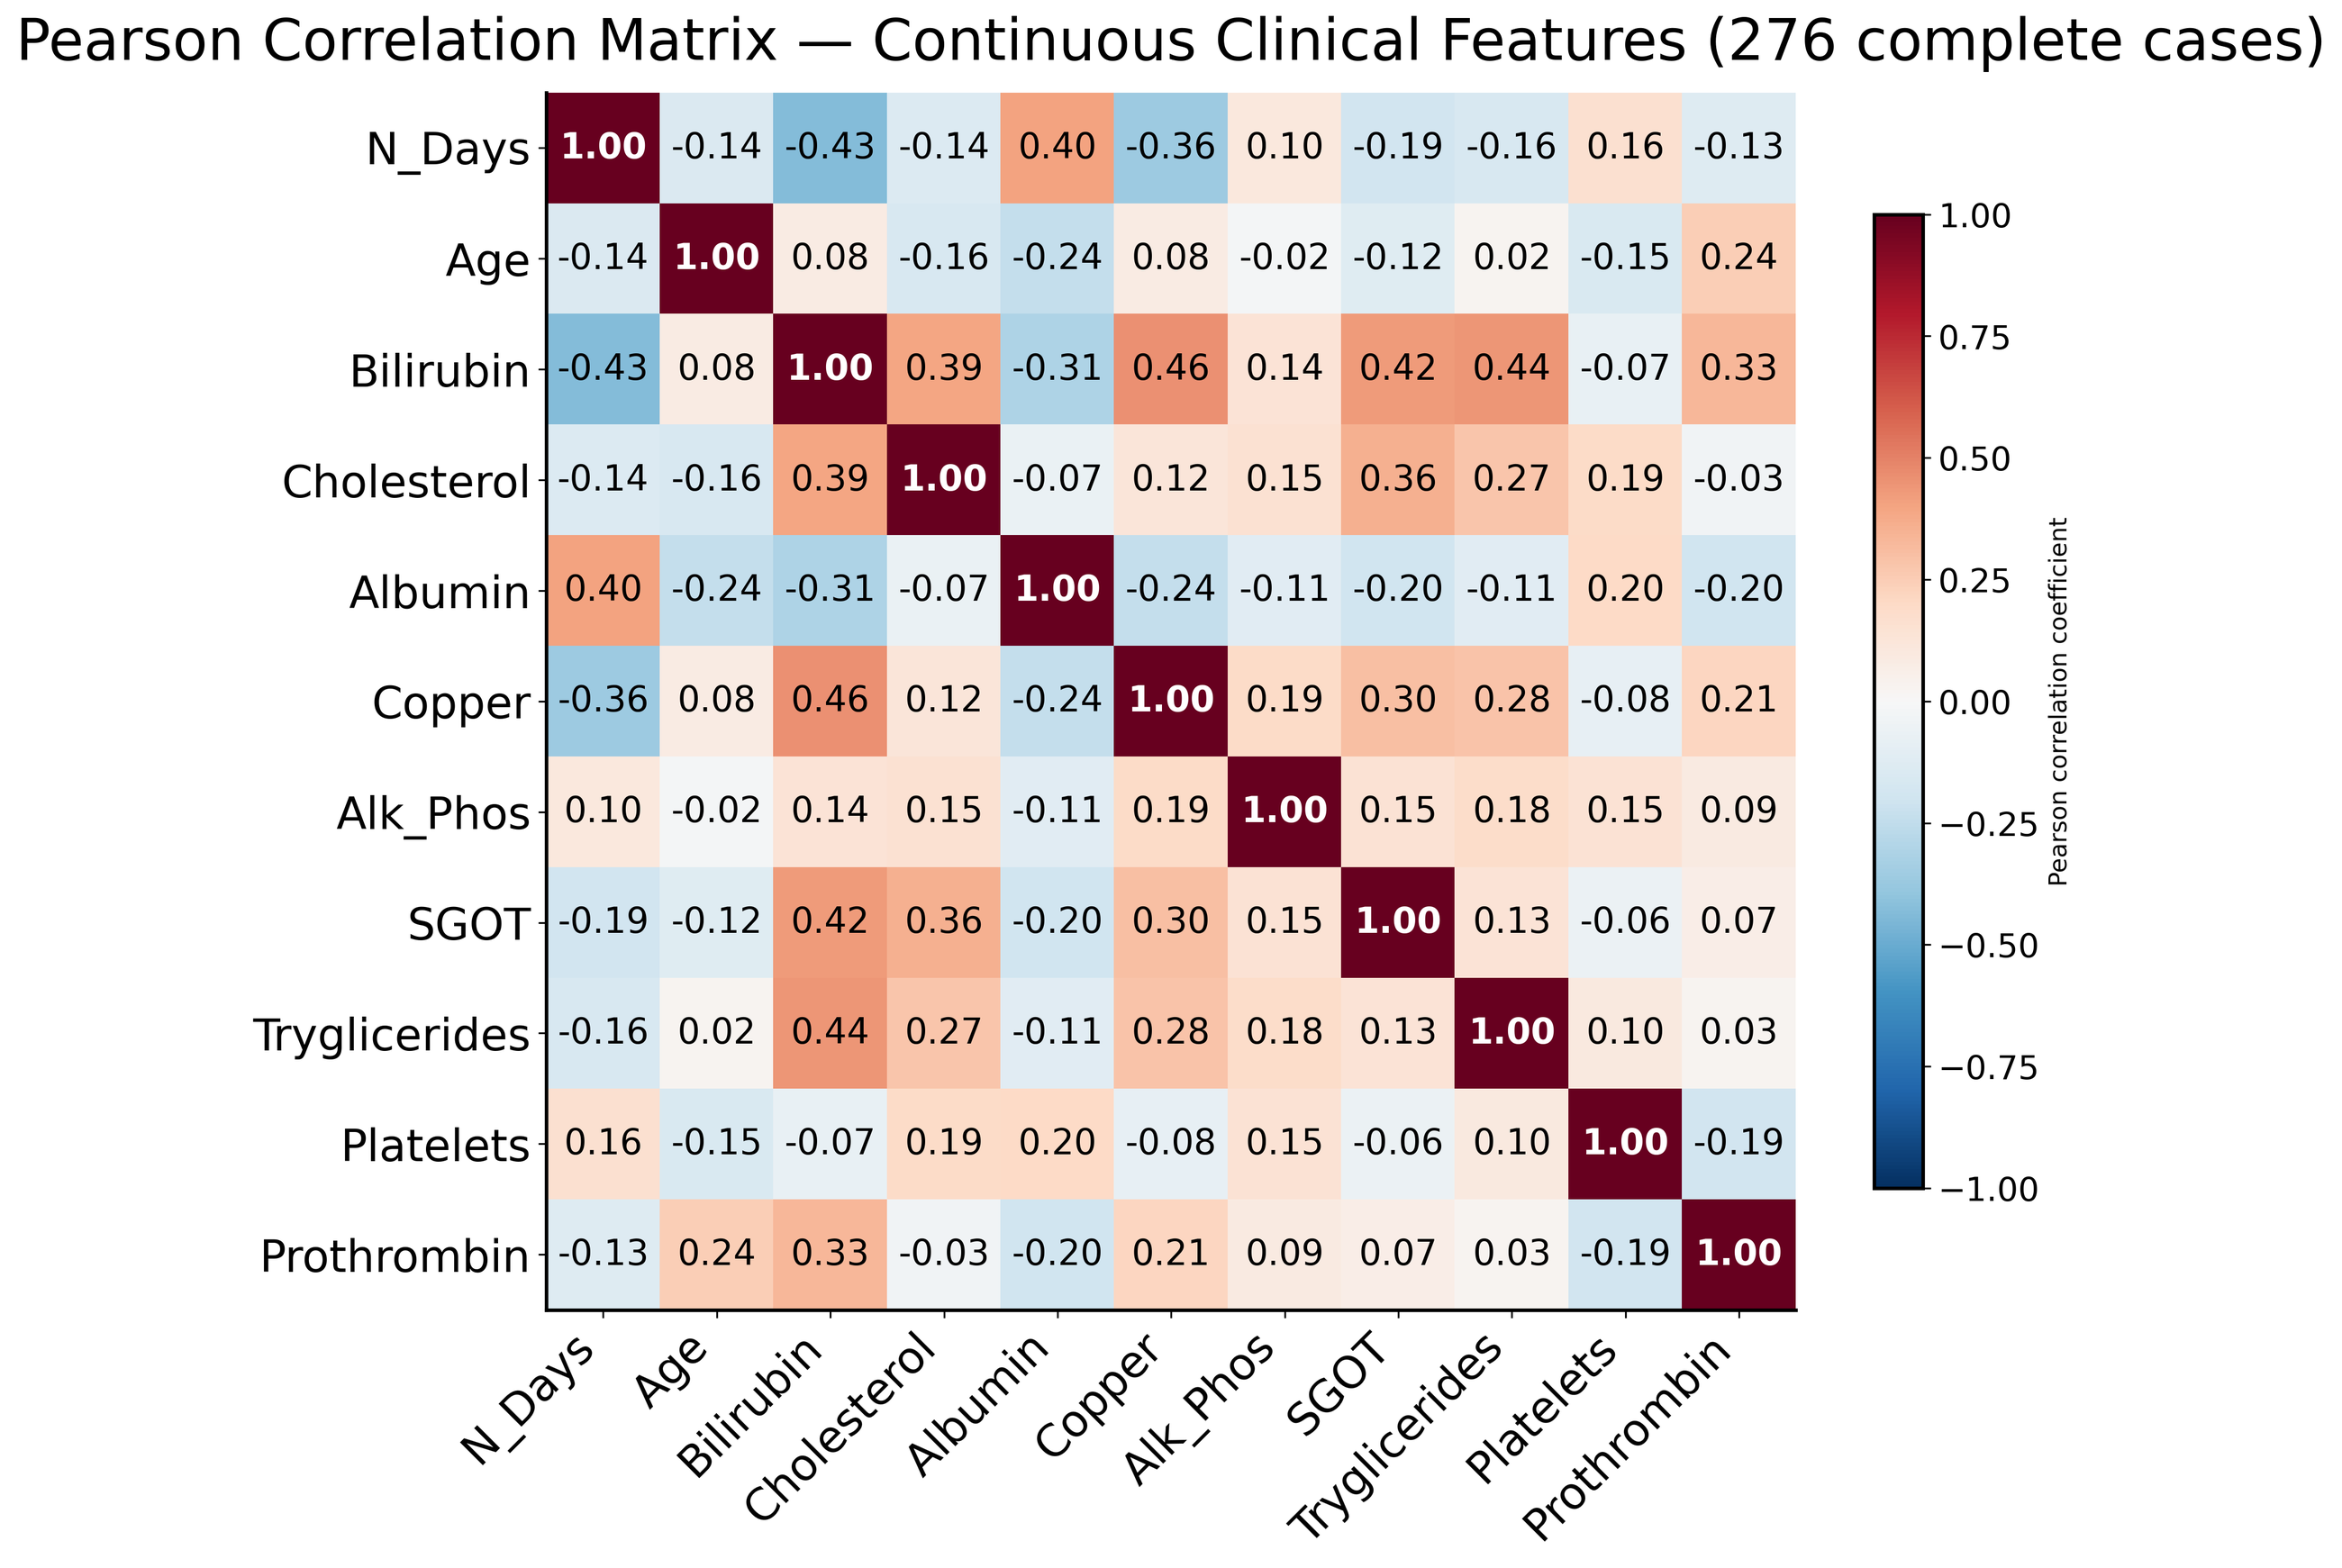
\includegraphics[width=0.68\linewidth]{figS01_correlation_matrix.png}
  \caption{Pearson correlation matrix across all 276 complete cases. Bilirubin correlates positively with Copper ($r = 0.46$), SGOT ($r = 0.42$), Cholesterol ($r = 0.39$) and Prothrombin ($r = 0.33$), reflecting the interlinked nature of hepatic synthetic and excretory function in PBC. N\_Days correlates negatively with Bilirubin ($r = -0.43$) and Copper ($r = -0.36$), consistent with more severe biochemical profiles being associated with shorter survival.}
  \label{figS:corrmatrix}
\end{figure}



\subsection{Generative Architectures}

Table~\ref{tab:arch} gives the complete specification of all three models. All are implemented directly in TensorFlow~2.15 without third-party synthetic-data libraries, which means every architectural choice is visible and auditable rather than inherited from a package default.

\begin{table}[!t]
  \centering
  \caption{Complete Architecture and Optimiser Settings for the Three Generative Models}
  \label{tab:arch}
  \resizebox{\columnwidth}{!}{%
  \begin{tabular}{llll}
    \toprule
    Setting & Vanilla GAN & cGAN & VAE \\
    \midrule
    Latent dimension      & 100          & 100 + 2 (one-hot) & 32 \\
    Encoder / discriminator & 256, 128   & 256, 128          & 128, 64 \\
    Generator / decoder     & 128, 256   & 128, 256          & 64, 128 \\
    Hidden activation     & LeakyReLU (0.2) & LeakyReLU (0.2) & ReLU \\
    Output activation     & Sigmoid      & Sigmoid           & Sigmoid \\
    Output dimension      & 18           & 18                & 18 \\
    Batch normalisation   & Yes (0.8)    & Yes (0.8)         & No \\
    Dropout               & 0.3 (disc.)  & 0.3 (disc.)       & No \\
    Optimiser             & Adam         & Adam              & Adam \\
    Learning rate         & $2\times10^{-4}$ & $2\times10^{-4}$ & $1\times10^{-3}$ \\
    $\beta_1$             & 0.5          & 0.5               & default \\
    Batch size            & 32           & 32                & 32 \\
    Epochs                & 500          & 300               & 300 \\
    Conditioning          & None         & Outcome label     & None \\
    Loss                  & Adversarial  & Adversarial       & ELBO ($\beta = 1.0$) \\
    Records generated     & 500          & 500               & 500 \\
    \bottomrule
  \end{tabular}%
  }
\end{table}

Both the cGAN and the VAE are named for what they are rather than after published models they resemble, and the distinction matters when comparing these results against the literature.

The model labelled cGAN is a conditional GAN in the sense of Mirza and Osindero \cite{mirza2014}: it conditions generator and discriminator on the outcome label and nothing more. It is deliberately not called CTGAN, because it implements none of the three components that define the Conditional Tabular GAN of Xu et al.\ \cite{xu2019}, namely mode-specific normalisation, training-by-sampling, and a PacGAN critic with the Wasserstein gradient penalty. A full CTGAN was implemented separately and compared against it; that comparison is reported in Section~IV of the main paper, where CTGAN reaches FID 0.108 against 0.072 for the cGAN after 4{,}000 generator updates, likely short of full convergence at this cohort size.

The model labelled VAE is likewise a standard variational autoencoder applied to min-max scaled tabular data. It is not the TVAE of Xu et al.\ \cite{xu2019}, which shares that paper's mode-specific normalisation, and results reported here should not be read as a benchmark of TVAE as originally specified.

Training curves for all three models are shown in Fig.~\ref{figS:training}. The adversarial losses settle without the sustained oscillation that signals mode collapse, and the VAE evidence lower bound falls steeply before levelling off, so all three models reach convergence within their training budgets.
\begin{figure}[!tb]
  \centering
  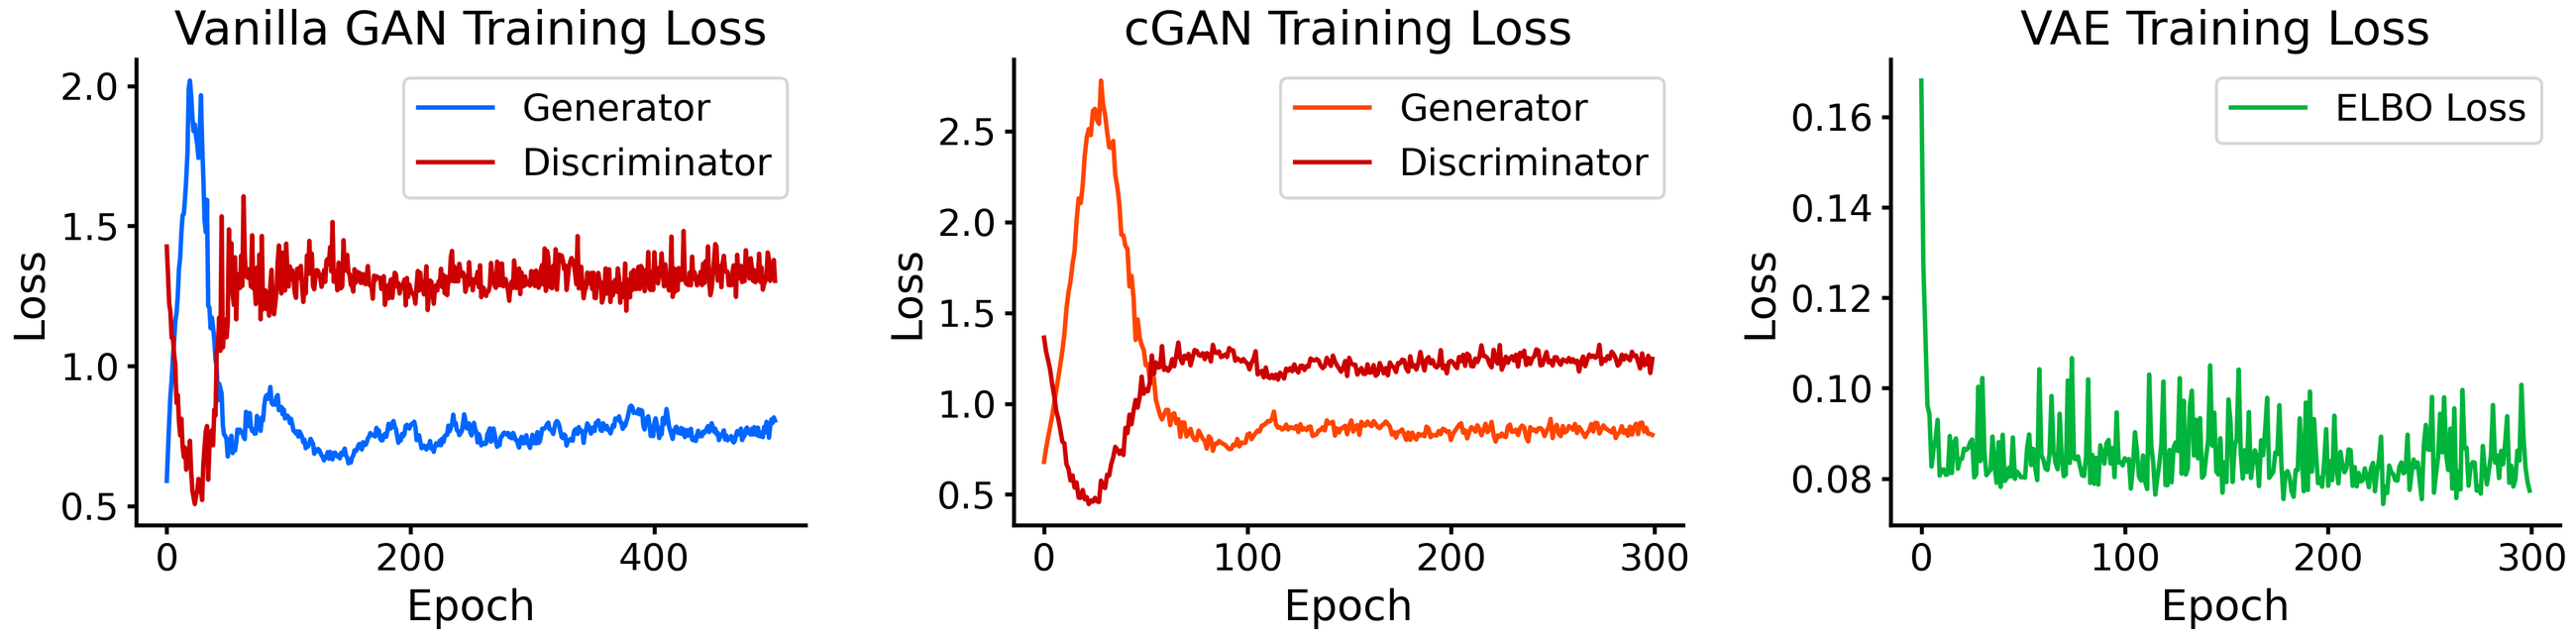
\includegraphics[width=\linewidth]{figS02_training_losses.png}
  \caption{Training loss curves. Left: Vanilla GAN generator and discriminator losses over 500 epochs. Centre: conditional GAN losses over 300 epochs. Right: VAE evidence lower bound over 300 epochs. The adversarial losses settle without sustained oscillation, indicating that mode collapse did not occur, and the VAE objective levels off well before its epoch budget is exhausted.}
  \label{figS:training}
\end{figure}



\subsection{Reproducibility}

Every result in the main paper and in this document comes from a single seeded execution of \texttt{master\_runner.py}. Python's \texttt{random}, NumPy, and TensorFlow are all seeded at 42, as is the train/test split, every scikit-learn estimator, and the SMOTE resampler. Re-executing the pipeline on the same machine and software environment reproduces all 19 result tables byte for byte, which we verified by checksum after a full clean re-run. TensorFlow does not guarantee bitwise-identical arithmetic across different hardware, operating systems or thread configurations, so small numerical differences may appear elsewhere; the conclusions do not depend on them.

Two practical notes for anyone reproducing this work. First, the consensus procedure used throughout is the \emph{equalised} variant described in Section~III of the main paper, in which the VAE pool is downsampled to match the smallest adversarial pool before voting. An earlier non-equalised variant produces a differently sized consensus set and different downstream numbers. Second, the nearest-neighbour privacy analysis reads the datasets written by \texttt{master\_runner.py} rather than regenerating them, so it always describes the same synthetic records the rest of the results are computed from.

% ===============================================================
\section{Complete Distributional Fidelity Results}

The main paper summarises distributional fidelity with a single aggregate FID per method and quotes a few representative Kolmogorov-Smirnov statistics. That summary hides an important structure, which the full tables make visible: the methods do not fail uniformly across features, and the method with the best aggregate score is not the best on every feature.

\subsection{Kolmogorov-Smirnov Tests}

Table~\ref{tab:ks} gives the two-sample KS statistic between each synthetic pool and the real training data, for all 11 continuous features.

\begin{table}[!t]
  \centering
  \caption{Two-Sample Kolmogorov-Smirnov Statistics Against Real Training Data. Lower is Better. An Asterisk Marks a Statistically Significant Difference at $\alpha = 0.05$}
  \label{tab:ks}
  \resizebox{\columnwidth}{!}{%
  \begin{tabular}{lcccc}
    \toprule
    Feature & GAN & cGAN & VAE & Consensus \\
    \midrule
    N\_Days & 0.194$^{*}$ & 0.075 & 0.396$^{*}$ & 0.209$^{*}$ \\
    Age & 0.083 & 0.122 & 0.410$^{*}$ & 0.214$^{*}$ \\
    Bilirubin & 0.413$^{*}$ & 0.487$^{*}$ & 0.485$^{*}$ & 0.269$^{*}$ \\
    Cholesterol & 0.308$^{*}$ & 0.454$^{*}$ & 0.341$^{*}$ & 0.172$^{*}$ \\
    Albumin & 0.315$^{*}$ & 0.079 & 0.389$^{*}$ & 0.194$^{*}$ \\
    Copper & 0.262$^{*}$ & 0.286$^{*}$ & 0.420$^{*}$ & 0.174$^{*}$ \\
    Alk\_Phos & 0.506$^{*}$ & 0.409$^{*}$ & 0.423$^{*}$ & 0.249$^{*}$ \\
    SGOT & 0.165$^{*}$ & 0.072 & 0.425$^{*}$ & 0.171$^{*}$ \\
    Triglycerides & 0.081 & 0.179$^{*}$ & 0.301$^{*}$ & 0.122$^{*}$ \\
    Platelets & 0.149$^{*}$ & 0.148$^{*}$ & 0.405$^{*}$ & 0.190$^{*}$ \\
    Prothrombin & 0.092 & 0.116 & 0.352$^{*}$ & 0.133$^{*}$ \\
    \bottomrule
  \end{tabular}%
  }
\end{table}

Three observations follow. The VAE differs significantly from the real data on all 11 features, which is consistent with its poor aggregate FID of 0.2280 and reflects the over-smoothing characteristic of variational reconstruction. The adversarial models each pass on a handful of features and fail badly on the heavily right-skewed ones: both GAN and cGAN produce their worst statistics on Bilirubin, Cholesterol and Alkaline Phosphatase, the three most skewed biomarkers in the cohort. This is the expected failure mode, since a sigmoid output layer trained on min-max scaled data has difficulty reproducing a long right tail.

The consensus set behaves differently from either of its parents. It is significant on all 11 features, so by the binary reading of the test it looks worse than the individual adversarial pools. But its \emph{magnitudes} are the most uniform of any method, and on the hardest features it is substantially the best: Bilirubin 0.269 against the GAN's 0.413 and cGAN's 0.487, and Alkaline Phosphatase 0.249 against 0.506 and 0.409. Cross-model agreement trades a small loss on the easy features for a large gain on the difficult ones. This is worth stating carefully, because it is the clearest evidence that consensus voting does what it was designed to do at the distributional level, even though Section~IV of the main paper shows it delivers no predictive benefit.

\subsection{Jensen-Shannon Divergence}

Table~\ref{tab:jsd} reports the Jensen-Shannon divergence per feature, which is bounded in $[0,1]$ and, unlike the KS statistic, is sensitive to differences across the whole distribution rather than at the point of maximum separation.

\begin{table}[!t]
  \centering
  \caption{Jensen-Shannon Divergence Between Synthetic and Real Training Distributions. Lower is Better}
  \label{tab:jsd}
  \resizebox{\columnwidth}{!}{%
  \begin{tabular}{lcccc}
    \toprule
    Feature & GAN & cGAN & VAE & Consensus \\
    \midrule
    N\_Days & 0.070 & 0.039 & 0.401 & 0.098 \\
    Age & 0.056 & 0.064 & 0.397 & 0.110 \\
    Bilirubin & 0.072 & 0.077 & 0.248 & 0.057 \\
    Cholesterol & 0.084 & 0.150 & 0.140 & 0.057 \\
    Albumin & 0.091 & 0.040 & 0.304 & 0.065 \\
    Copper & 0.063 & 0.069 & 0.250 & 0.071 \\
    Alk\_Phos & 0.138 & 0.110 & 0.205 & 0.080 \\
    SGOT & 0.033 & 0.030 & 0.325 & 0.062 \\
    Triglycerides & 0.021 & 0.048 & 0.179 & 0.039 \\
    Platelets & 0.045 & 0.055 & 0.356 & 0.095 \\
    Prothrombin & 0.023 & 0.030 & 0.219 & 0.047 \\
    \bottomrule
  \end{tabular}%
  }
\end{table}

The divergence measure tells a cleaner story than the KS test. The VAE is between three and ten times worse than every other method on nearly every feature, with N\_Days and Age the worst affected at roughly 0.40. The consensus set is the most consistent performer: it never exceeds 0.110 on any feature, whereas the GAN reaches 0.138 on Alkaline Phosphatase and cGAN reaches 0.150 on Cholesterol. Averaged across features the consensus set is the best of the four, which is the result the aggregate FID of 0.0809 also reflects.

\subsection{Standardised Mean Differences}

Table~\ref{tab:cohens} gives Cohen's $d$ between each synthetic pool and the real training data. A positive value means the synthetic mean exceeds the real mean.

\begin{table}[!t]
  \centering
  \caption{Cohen's $d$ Between Synthetic and Real Training Data. Values Near Zero Indicate Well-Matched Means}
  \label{tab:cohens}
  \resizebox{\columnwidth}{!}{%
  \begin{tabular}{lcccc}
    \toprule
    Feature & GAN & cGAN & VAE & Consensus \\
    \midrule
    N\_Days & $-0.245$ & $+0.100$ & $+0.099$ & $-0.025$ \\
    Age & $-0.012$ & $+0.007$ & $-0.072$ & $+0.076$ \\
    Bilirubin & $+0.686$ & $+0.695$ & $-0.016$ & $+0.530$ \\
    Cholesterol & $+0.581$ & $+0.661$ & $-0.044$ & $+0.426$ \\
    Albumin & $-0.644$ & $+0.059$ & $+0.163$ & $-0.193$ \\
    Copper & $+0.607$ & $+0.546$ & $-0.104$ & $+0.462$ \\
    Alk\_Phos & $+0.771$ & $+0.667$ & $-0.025$ & $+0.531$ \\
    SGOT & $+0.362$ & $+0.089$ & $-0.230$ & $+0.108$ \\
    Triglycerides & $+0.229$ & $+0.303$ & $+0.017$ & $+0.281$ \\
    Platelets & $+0.248$ & $+0.175$ & $-0.088$ & $+0.067$ \\
    Prothrombin & $+0.159$ & $+0.227$ & $-0.045$ & $+0.197$ \\
    \bottomrule
  \end{tabular}%
  }
\end{table}

This table contains the most counterintuitive result in the supplementary material, and it deserves attention. By the standardised mean difference criterion the VAE is the \emph{best} method: every one of its 11 values is negligible, none exceeding 0.230 in magnitude. The adversarial models systematically overshoot on the skewed biomarkers, with the GAN reaching $+0.771$ on Alkaline Phosphatase.

The explanation is that a variational autoencoder trained to minimise reconstruction error will reproduce the mean of the training distribution almost exactly while collapsing its variance and shape. Matching the first moment is not the same as matching the distribution. The KS and Jensen-Shannon results in Tables~\ref{tab:ks} and~\ref{tab:jsd} show the VAE failing comprehensively on distributional shape at the same time as it succeeds on means.

The practical lesson generalises well beyond this dataset: a single fidelity metric can be satisfied by a model that is wrong in every other respect, and a method that looks best under one criterion can look worst under another computed on the same data. Reporting one number invites exactly this error. It is the distributional analogue of the main paper's central finding, that distributional similarity and predictive utility are different properties that must be measured separately.

\subsection{Supporting Figures}

Fig.~\ref{figS:iqr} shows the IQR-based Tukey fence filter (Section~III of the main paper) in action on the Bilirubin distribution, the hardest continuous feature to reproduce faithfully.

Four further figures make the tables above visible. Fig.~\ref{figS:distributions} plots the marginal distributions of six representative biomarkers side by side for all four synthetic datasets. It shows directly what the KS statistics in Table~\ref{tab:ks} quantify: the adversarial models track the real distribution closely on Albumin and Prothrombin, while every method struggles on the heavily right-skewed Bilirubin, and the VAE distribution is displaced rather than merely broadened.

\begin{figure}[!tb]
  \centering
  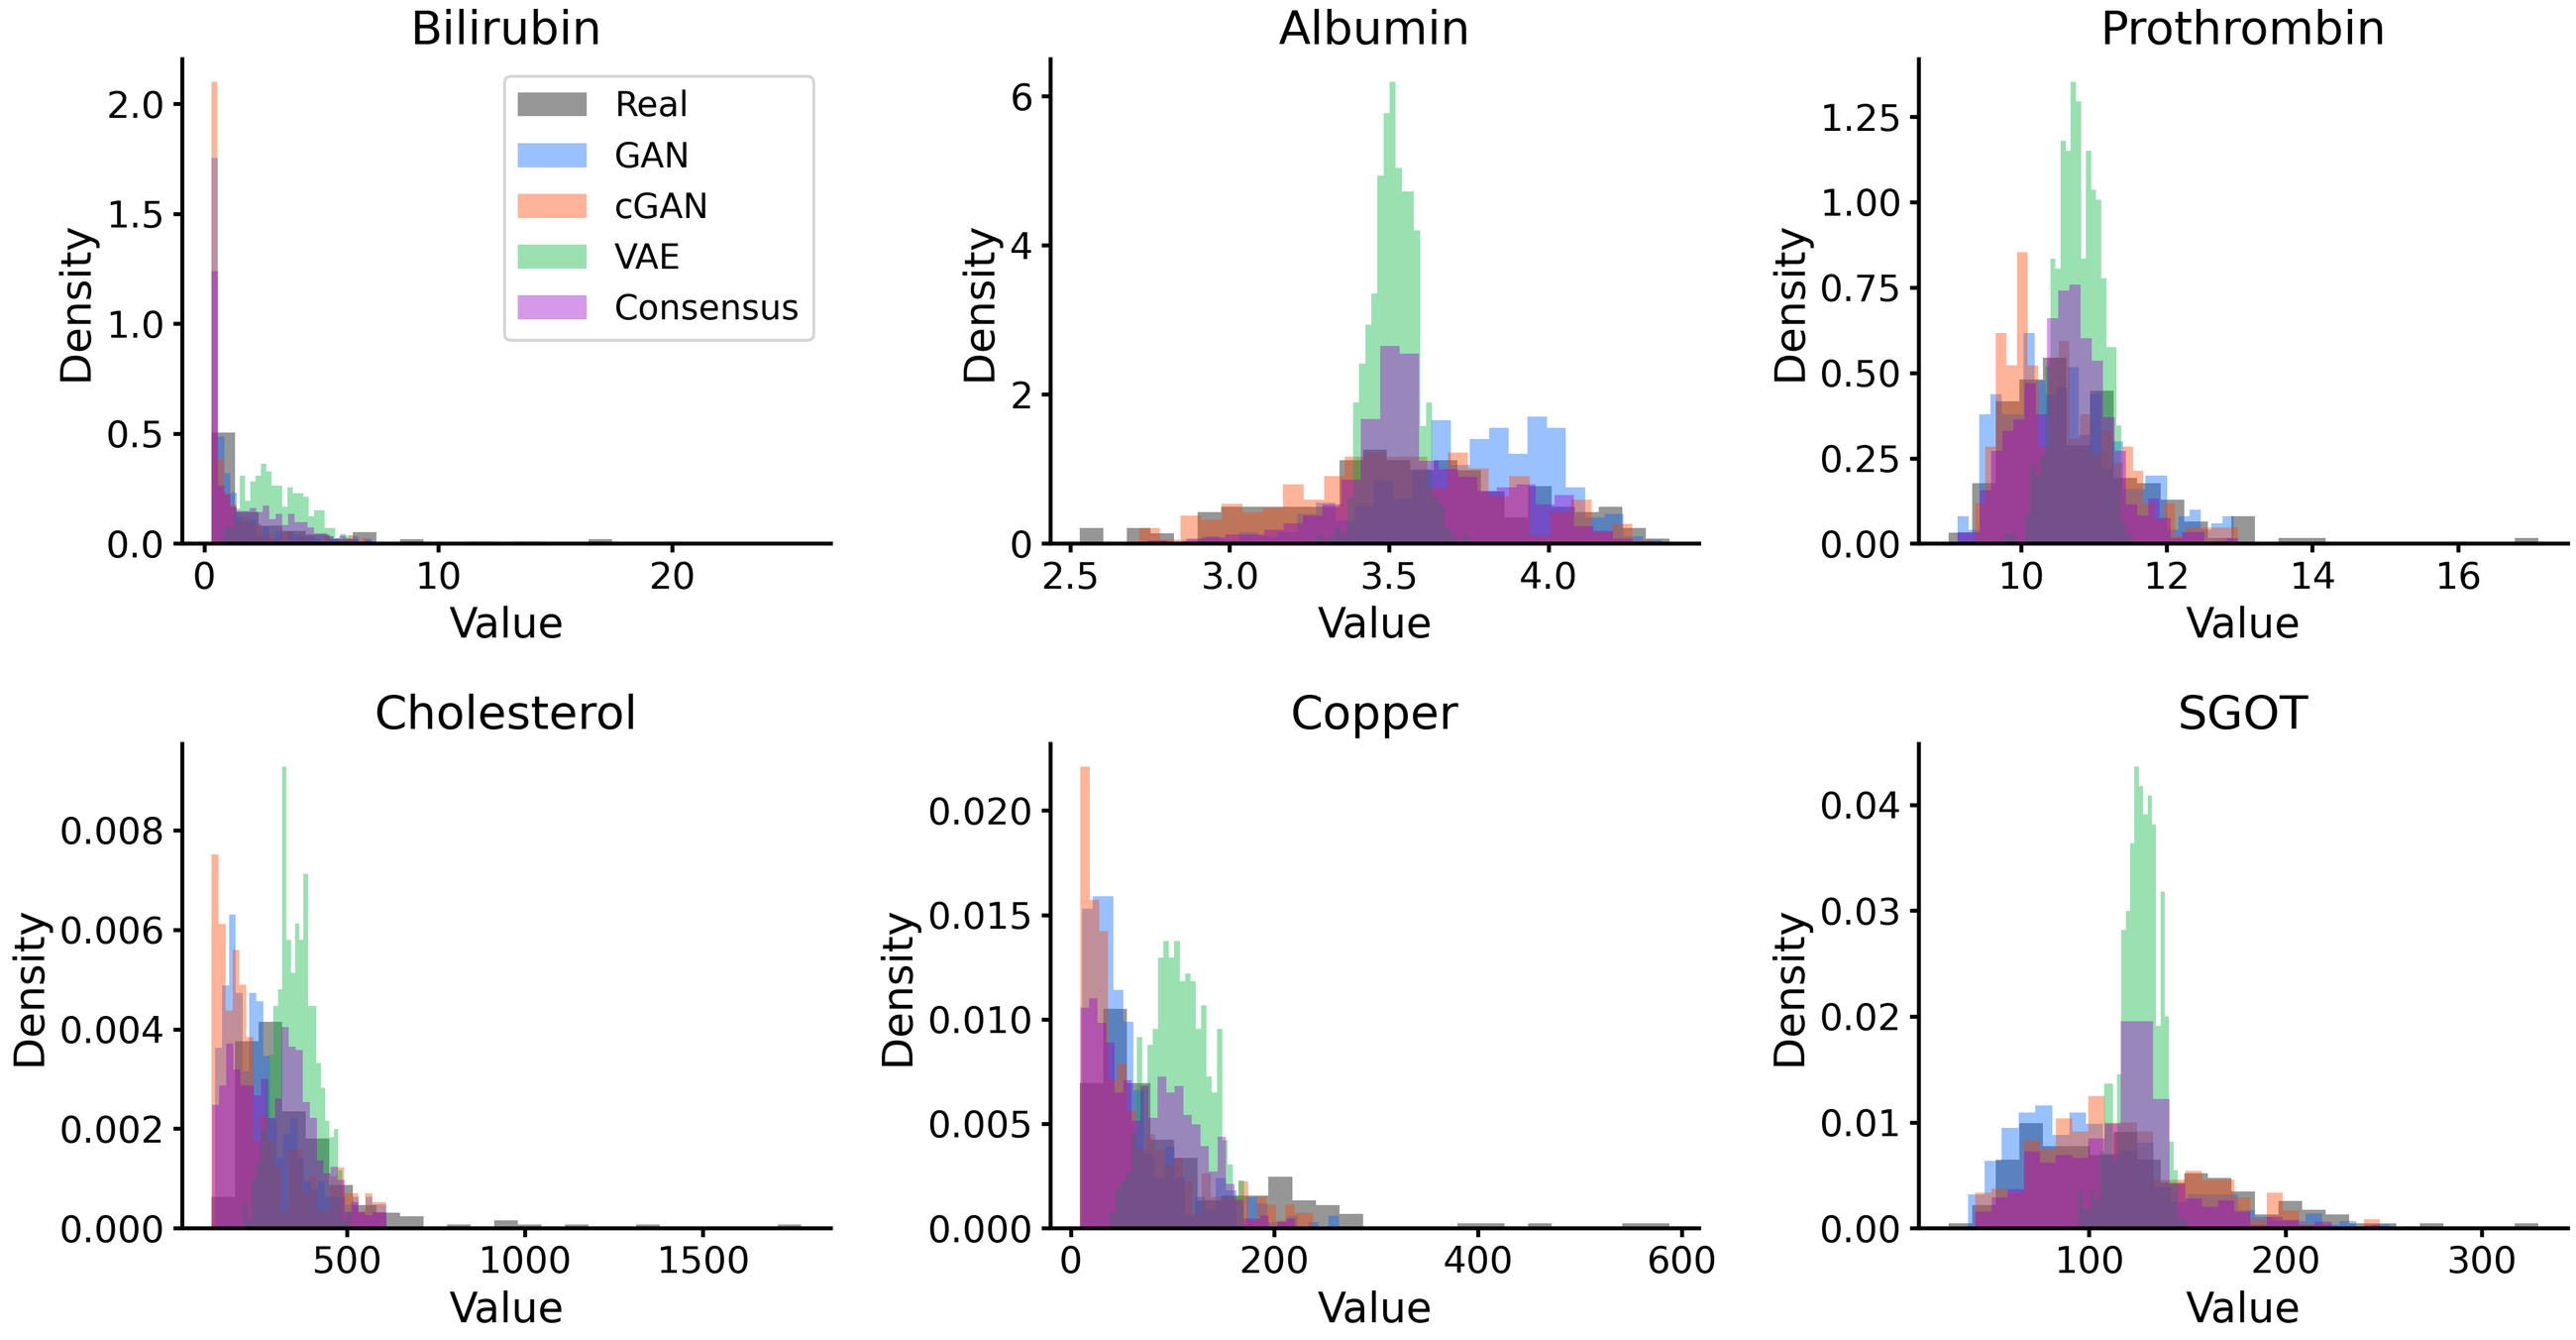
\includegraphics[width=0.88\linewidth]{figS03_distribution_comparison.png}
  \caption{Marginal distributions of six representative biomarkers for real training data and all four synthetic datasets. GAN and cGAN reproduce Albumin and Prothrombin closely. All methods diverge on the heavily right-skewed Bilirubin and Cholesterol, and the VAE distribution for Bilirubin is shifted noticeably rightward, matching the KS statistics in Table~\ref{tab:ks}.}
  \label{figS:distributions}
\end{figure}

Fig.~\ref{figS:corrcomparison} moves from single features to their joint structure, comparing the real correlation matrix against the consensus set. The dominant clinical associations survive generation, but the weaker off-diagonal terms are attenuated, which is the expected signature of a generator that has learned the strongest dependencies and smoothed the rest.

\begin{figure}[!tb]
  \centering
  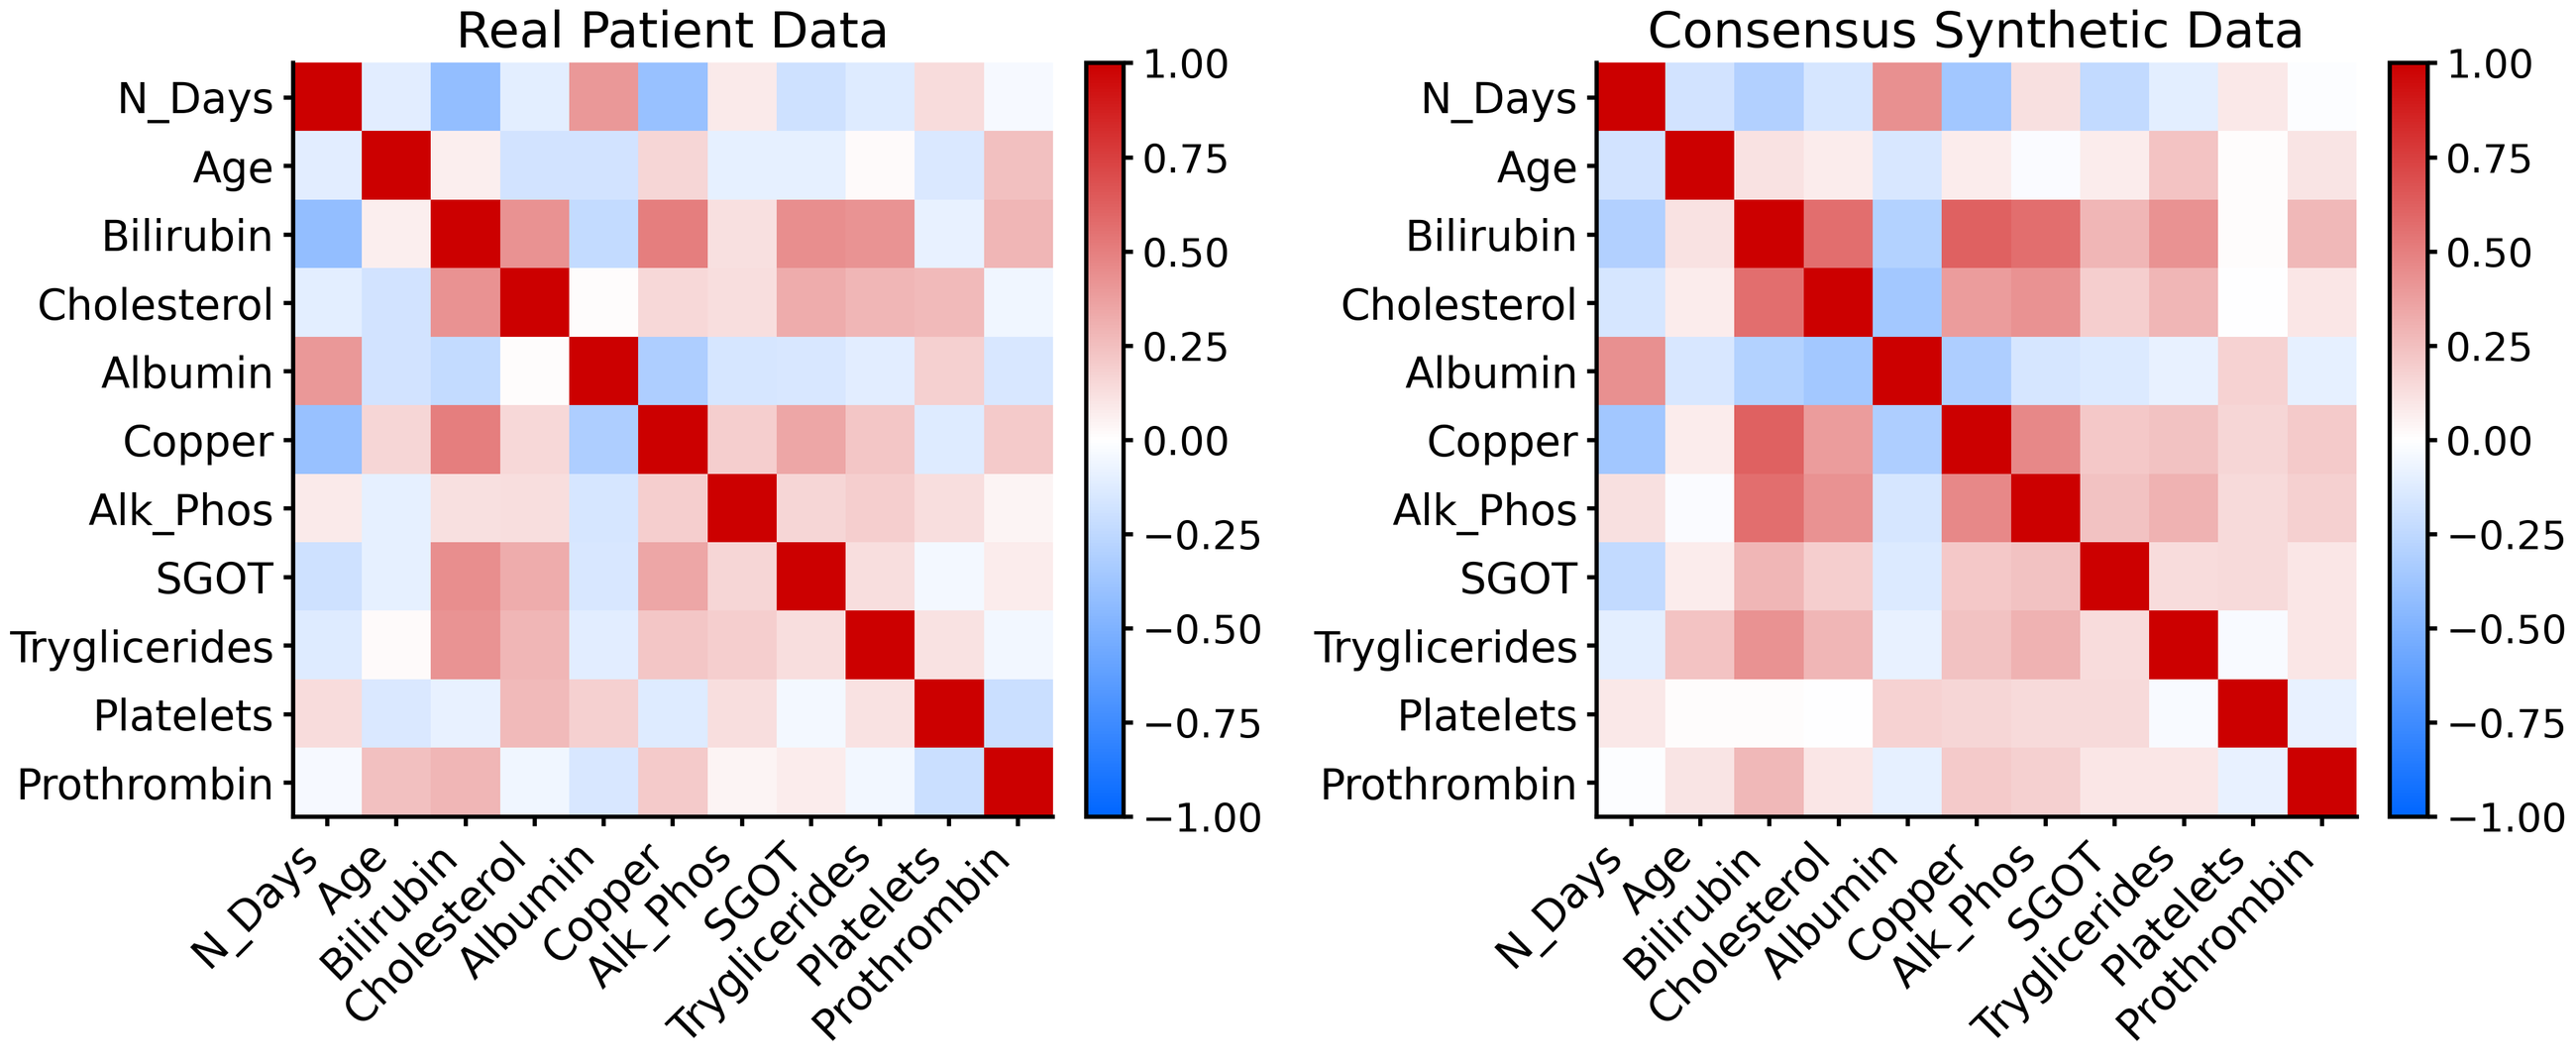
\includegraphics[width=\linewidth]{figS04_correlation_heatmap.png}
  \caption{Pearson correlation structure of real training data (left) against the equalised consensus set (right). Dominant clinical associations are preserved, including the positive Bilirubin-Copper and negative N\_Days-Bilirubin relationships, while weaker correlations are attenuated.}
  \label{figS:corrcomparison}
\end{figure}

Fig.~\ref{figS:tsne} projects real and synthetic records into two dimensions. The consensus set concentrates in the centre of the real manifold rather than spreading across it. That single geometric fact explains two results at once: the good aggregate distributional scores, because the centre is where most real patients are, and the poor privacy profile in Table~II of the main paper, because the centre is also where real patients are easiest to sit close to.

\begin{figure}[!tb]
  \centering
  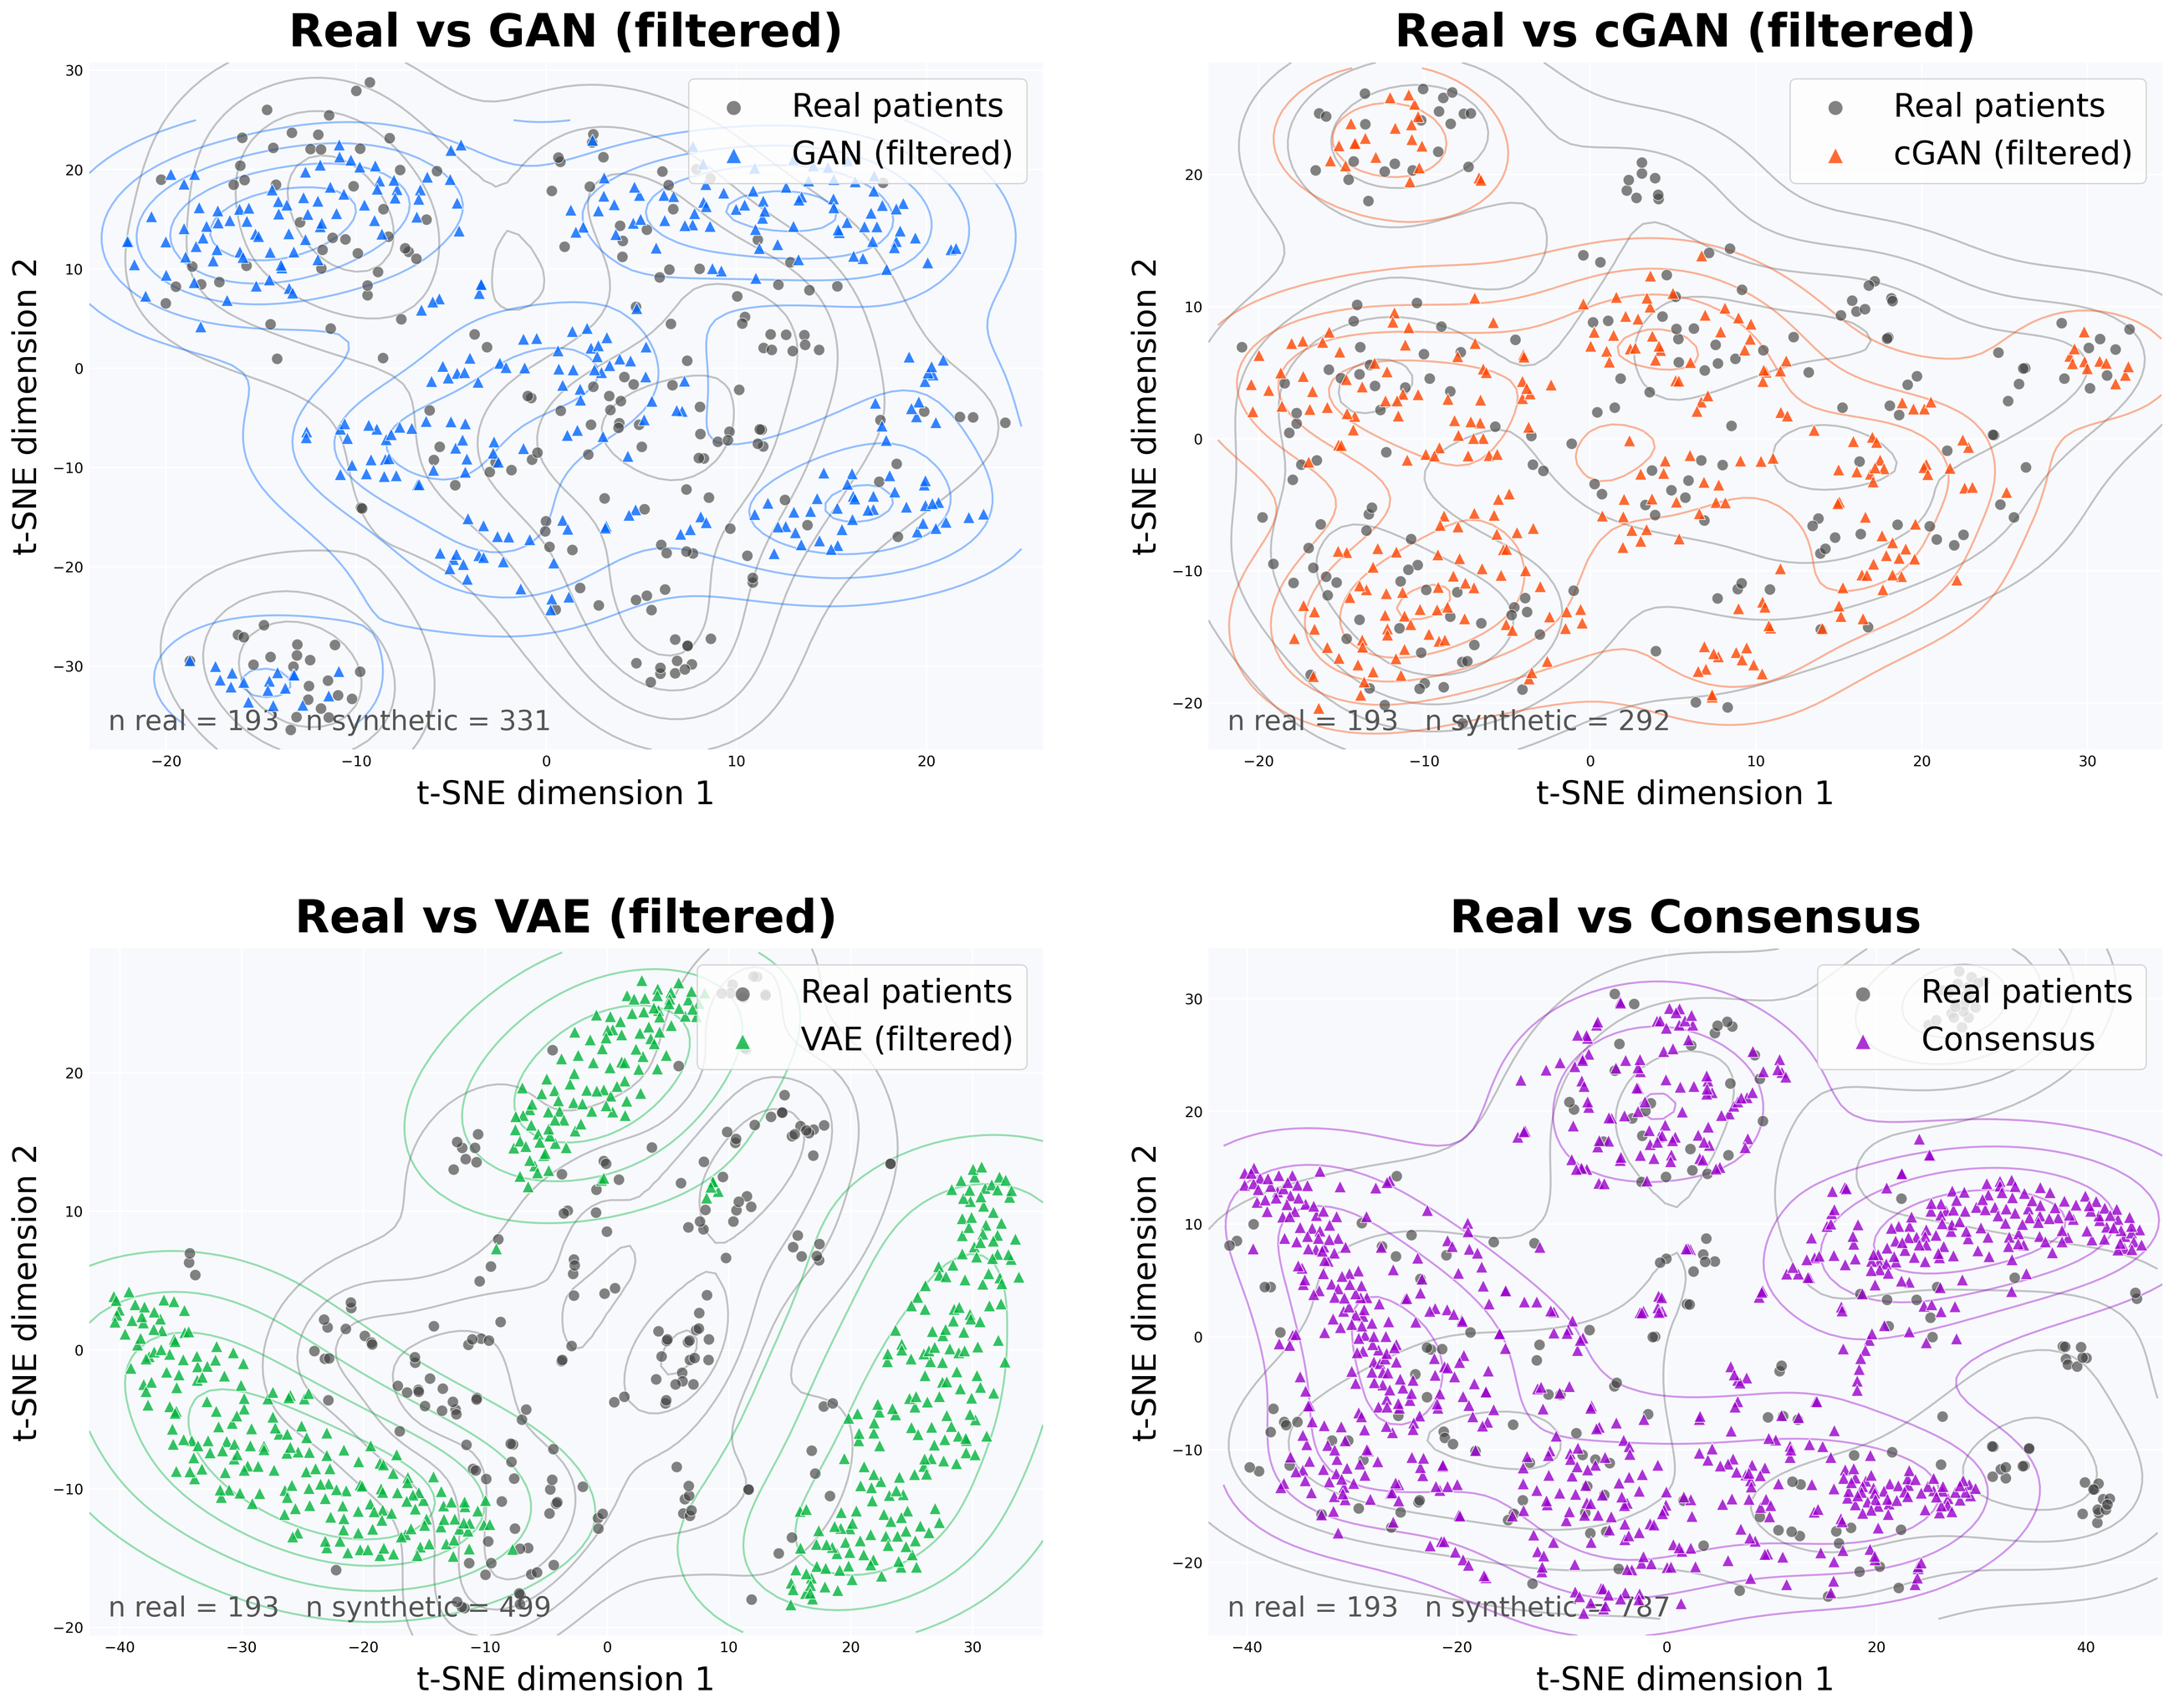
\includegraphics[width=0.58\linewidth]{figS05_tsne_projection.png}
  \caption{t-SNE projection of real patients and each synthetic method from the original 18-dimensional feature space. Filtered GAN and cGAN records overlap the real manifold. VAE records spread beyond the real density contours. The consensus set concentrates in the central high-density region, which explains both its favourable distributional scores and its elevated near-duplicate rate of 21.1\% reported in Table~II of the main paper.}
  \label{figS:tsne}
\end{figure}

% ===============================================================
\section{Consensus Threshold Sensitivity}

The consensus tolerance of 5.0 standardised units is the single most consequential free parameter in the pipeline, so it was selected by a systematic sweep rather than by inspection. Table~\ref{tab:threshold} reports the sweep across eight values.

\begin{table}[!t]
  \centering
  \caption{Consensus Tolerance Sweep. Composition Percentages Are Shares of the Accepted Set. The Real Training Cohort Is 40.4\% Deceased}
  \label{tab:threshold}
  \resizebox{\columnwidth}{!}{%
  \begin{tabular}{ccccccc}
    \toprule
    Tol. & Records & GAN \% & cGAN \% & VAE \% & Deceased \% & FID \\
    \midrule
    2.5 & 89 & 11.2 & 15.7 & 73.0 & 1.1 & 0.2262 \\
    3.0 & 252 & 20.6 & 15.1 & 64.3 & 10.7 & 0.1677 \\
    3.5 & 461 & 21.5 & 16.1 & 62.5 & 17.4 & 0.1441 \\
    4.0 & 667 & 22.6 & 17.4 & 60.0 & 21.1 & 0.1247 \\
    4.5 & 848 & 23.5 & 20.8 & 55.8 & 23.2 & 0.1061 \\
    5.0 & 953 & 25.1 & 22.6 & 52.4 & 24.7 & 0.0950 \\
    5.5 & 1017 & 27.4 & 23.5 & 49.1 & 25.8 & 0.0864 \\
    6.0 & 1043 & 28.7 & 23.5 & 47.8 & 26.3 & 0.0829 \\
    \bottomrule
  \end{tabular}%
  }
\end{table}

The class-balance column is the reason a very tight tolerance is unusable. At 2.5 the accepted set is 1.1\% deceased, against 40.4\% in the real training cohort. A strict agreement requirement does not sample the outcome classes evenly: deceased patients occupy the sparser, more extreme region of biomarker space, exactly where three independently trained models are least likely to place records near one another. Tightening the tolerance therefore filters out the minority class almost entirely, and augmenting with such a set would worsen the imbalance the augmentation was meant to relieve.

As the tolerance widens, class balance recovers monotonically and FID improves monotonically, but the marginal return falls away. Between 5.0 and 6.0 the accepted set grows by 90 records while FID improves by only 0.0121, and each additional record is by construction one that fewer models agreed on. The value of 5.0 sits at the point where class balance has become tolerable at 24.7\% and the quality curve has begun to flatten. It is a defensible compromise rather than an optimum, and we state it as such.

Note that the record counts in this table are from the non-equalised voting procedure, which is why 5.0 yields 953 records here against the 787 reported in the main paper. The equalisation step, which downsamples the VAE pool before voting, is applied afterwards and reduces the count while improving fidelity.

% ===============================================================
\section{Extended Privacy Analyses}

Fig.~\ref{figS:privacyrisk} gives the full nearest-neighbour privacy risk analysis referenced in Section~IV of the main paper (near-duplicate rates in Table~II there).

\subsection{Output Perturbation}

The filtered VAE pool carries a 35.7\% near-duplicate rate, meaning more than one generated record in three sits closer to a real training patient than the 5th-percentile real-to-real distance. Releasing such a set would be indefensible. Table~\ref{tab:perturb} reports a sweep of post-hoc Gaussian perturbation applied to the eleven continuous features, with $\sigma$ expressed in units of each feature's training standard deviation.

\begin{table}[!t]
  \centering
  \caption{Gaussian Output Perturbation Applied to the Filtered VAE Pool ($n = 499$)}
  \label{tab:perturb}
  \begin{tabular}{cccc}
    \toprule
    $\sigma$ & Near-dup.\ ($n$) & Near-dup.\ (\%) & FID \\
    \midrule
    0.0 & 178 & 35.7 & 0.2280 \\
    0.1 & 169 & 33.9 & 0.2095 \\
    0.2 & 140 & 28.1 & 0.1720 \\
    0.3 & 88 & 17.6 & 0.1402 \\
    0.5 & 29 & 5.8 & 0.0804 \\
    0.7 & 7 & 1.4 & 0.0481 \\
    1.0 & 2 & 0.4 & 0.0319 \\
    \bottomrule
  \end{tabular}
\end{table}

Both columns improve together, which is not what one would expect. Adding noise to synthetic records normally buys privacy at the cost of fidelity; here FID improves from 0.2280 to 0.0481 while the near-duplicate rate falls from 35.7\% to 1.4\%.

The reason is specific to how the VAE fails. It does not produce a broadly correct distribution with a few risky records; it produces records clustered tightly around particular real patients, which is simultaneously why its near-duplicate rate is high and why its marginal distributions are too narrow. Perturbation attacks both problems at once, dispersing the clusters away from individual patients and widening the marginals back towards the real spread. The improvement is therefore a correction of a specific defect rather than a general free lunch, and it should not be expected to transfer to a generator whose failure mode is different.

We select $\sigma = 0.7$ rather than 1.0 because it already clears any reasonable near-duplicate target at 1.4\%, and pushing further begins to distort a distribution that has by then been corrected.

\subsection{Formal Differential Privacy}

Table~\ref{tab:dpsgd} reports estimated privacy budgets for differentially private stochastic gradient descent at $\delta = 10^{-5}$, across noise multipliers from 0.5 to 3.0, for the $n = 193$ training cohort.

\begin{table}[!t]
  \centering
  \caption{Estimated DP-SGD Privacy Budget at $\delta = 10^{-5}$ for $n = 193$ Training Patients}
  \label{tab:dpsgd}
  \begin{tabular}{ccl}
    \toprule
    Noise multiplier & $\varepsilon$ & Interpretation \\
    \midrule
    0.5 & 210.4 & Essentially no DP guarantee \\
    0.8 & 89.2 & Very weak privacy guarantee \\
    1.0 & 61.2 & Very weak privacy guarantee \\
    1.2 & 46.0 & Very weak privacy guarantee \\
    1.5 & 33.6 & Very weak privacy guarantee \\
    2.0 & 23.9 & Very weak privacy guarantee \\
    3.0 & 14.0 & Very weak privacy guarantee \\
    \bottomrule
  \end{tabular}
\end{table}

Values of $\varepsilon$ below roughly 10 are usually considered the threshold of a meaningful guarantee, and values below 1 are considered strong. Even at a noise multiplier of 3.0, which would severely damage a generative model trained on 193 records, the budget remains at 14.0. The conclusion is unambiguous and worth stating plainly: formal differential privacy is not attainable on a cohort of this size. The privacy budget scales with the number of training examples, and 193 is simply too few for the accounting to close at a defensible $\varepsilon$.

This is why the main paper recommends output perturbation as the practical mitigation at this scale, and treats DP-SGD as an option that becomes available only once a cohort of several hundred patients has been assembled. Reporting a DP-SGD result at $\varepsilon = 14$ as though it constituted a privacy guarantee would be misleading, and we avoid doing so.

Both analyses in this section are plotted together in Fig.~\ref{figS:privacyenhance}.

% ===============================================================
\section{Subgroup Analysis}

Table~\ref{tab:subgroup} reports test-set AUC within six clinical strata, comparing the real-only baseline against consensus augmentation, on the leak-free 17-feature input (N\_Days excluded). Each cell gives Scenario~A followed by Scenario~C.

\begin{table}[!t]
  \centering
  \caption{Subgroup Test-Set AUC, N\_Days Excluded, Reported as Scenario A / Scenario C. Subgroups Below $n = 20$ Are Reported for Completeness Only}
  \label{tab:subgroup}
  \resizebox{\columnwidth}{!}{%
  \begin{tabular}{lccccc}
    \toprule
    Subgroup & $n$ & Dec. & RF & GB & LR \\
    \midrule
    Early stage (1--2) & 17 & 4 & 0.587 / 0.596 & 0.615 / 0.596 & 0.635 / 0.654 \\
    Late stage (3--4) & 66 & 29 & 0.848 / 0.852 & 0.857 / 0.859 & 0.863 / 0.859 \\
    Female & 72 & 27 & 0.839 / 0.835 & 0.843 / 0.831 & 0.844 / 0.834 \\
    Male & 11 & 6 & 0.517 / 0.567 & 0.533 / 0.633 & 0.600 / 0.767 \\
    D-penicillamine & 39 & 17 & 0.765 / 0.763 & 0.778 / 0.775 & 0.818 / 0.856 \\
    Placebo & 44 & 16 & 0.884 / 0.891 & 0.877 / 0.864 & 0.853 / 0.842 \\
    \bottomrule
  \end{tabular}%
  }
\end{table}

Among the four subgroups large enough to support inference, the picture is consistent with the overall null result. Differences between Scenario~A and Scenario~C stay within about $\pm 0.04$, with no consistent direction, and every AUC exceeds 0.76. Augmentation neither helps nor harms in any stratum we can measure reliably.

The two small subgroups illustrate why we decline to interpret them. On the 11 male patients, all three classifiers move in the same direction this time (Random Forest 0.517 to 0.567, Gradient Boosting 0.533 to 0.633, Logistic Regression 0.600 to 0.767), which on six deceased patients is as consistent with a single reordered prediction shifting AUC by several points as with a real effect; the subgroup is too small to distinguish the two. The early-stage subgroup, with 17 patients and four deceased, is equally unstable and additionally sits near chance for all three classifiers.

We report these rows rather than dropping them because selective omission of inconvenient strata is itself a reporting problem. But no weight should be placed on them, and a reader who wishes to cite a subgroup result should use the late-stage, female, or treatment-arm rows.

% ===============================================================
\section{Graphical Views of the Predictive Results}

Every quantity plotted in this section also appears numerically in Tables~III and~IV of the main manuscript. These figures add no new evidence; they are included because a pattern across five scenarios and three classifiers is easier to read at a glance than to reconstruct from a table. Each is discussed in turn.

Fig.~\ref{figS:prcurves} gives Precision-Recall curves. PR curves matter for this cohort because the classes are imbalanced, at 78 deceased against 115 survivors in the training set, and PR is more sensitive than ROC to performance on the minority class. All three classifiers hold precision above 0.7 across a wide recall range, and the scenario curves sit close together, which is the same null visible in the ROC analysis.

\begin{figure}[!tb]
  \centering
  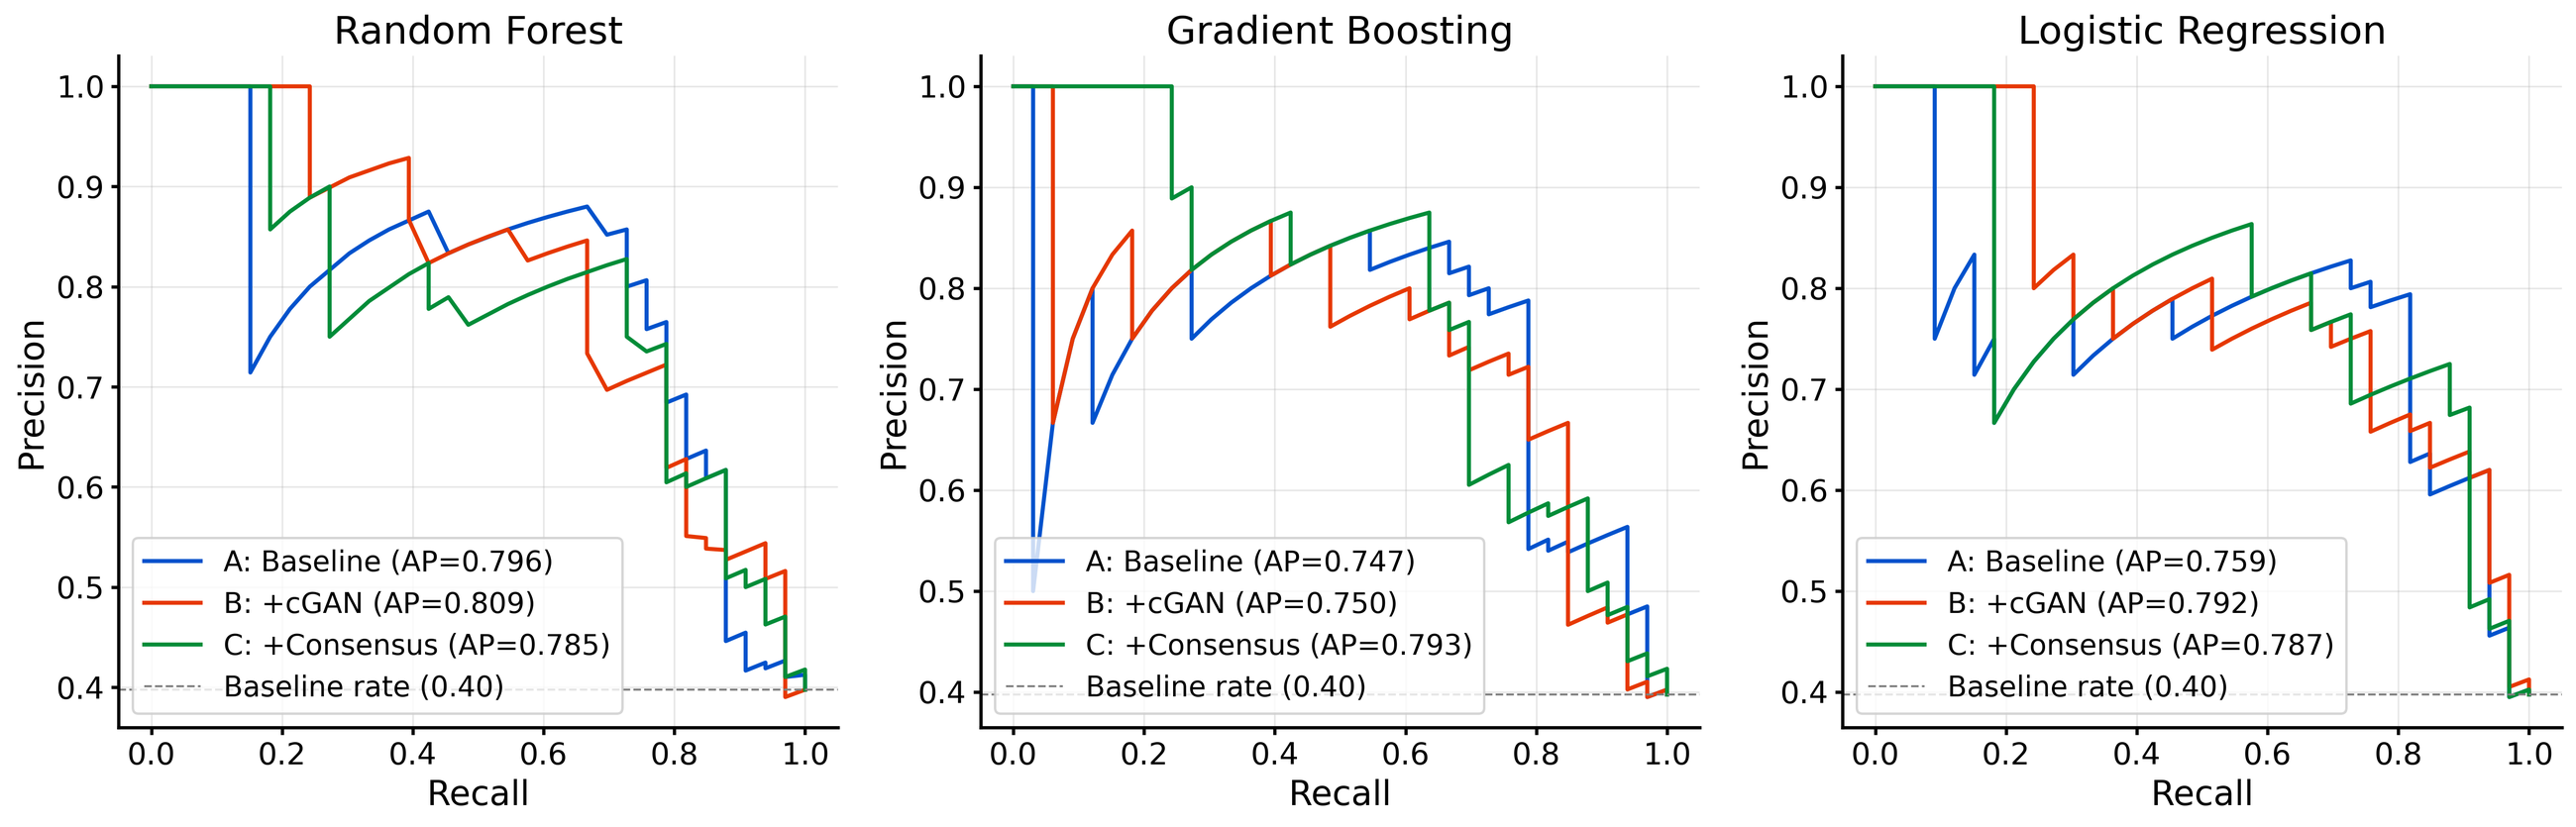
\includegraphics[width=\linewidth]{figS06_pr_curves.png}
  \caption{Precision-Recall curves by classifier and training scenario on the 83-patient real held-out test set. PR curves are informative for this cohort given its class imbalance of 78 deceased against 115 survivors in the training set. All classifiers hold precision above 0.7 across a wide recall range.}
  \label{figS:prcurves}
\end{figure}

Fig.~\ref{figS:auc} compares AUC directly across scenarios. Every combination clears the 0.8 threshold conventionally taken as good discrimination, so no augmentation strategy damages the model. Equally, none lifts it: the tallest bar in each classifier group is the baseline or within noise of it.

\begin{figure}[!tb]
  \centering
  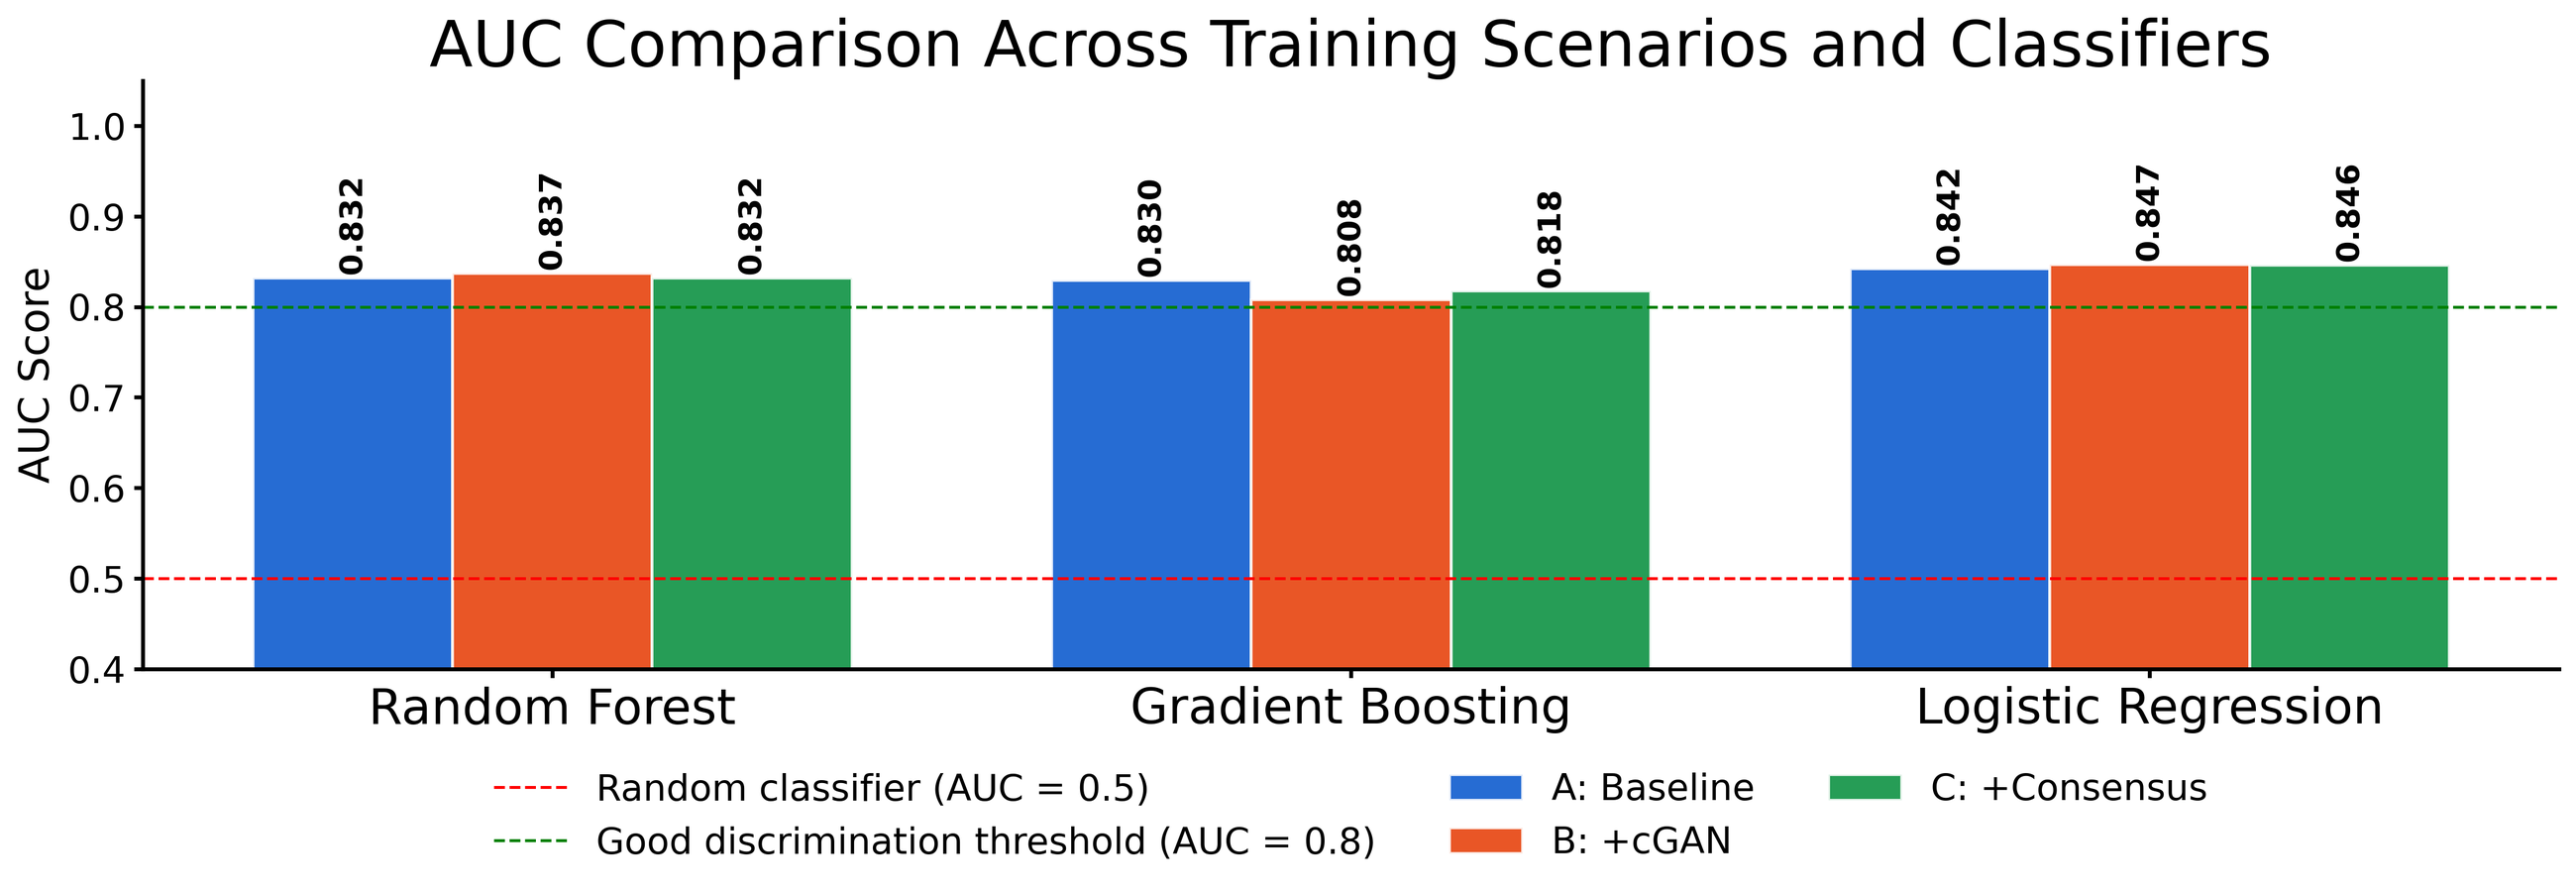
\includegraphics[width=\linewidth]{figS07_auc_comparison.png}
  \caption{AUC across all three classifiers for scenarios A, B and C, N\_Days excluded from classifier input. The green dashed line marks AUC~$= 0.8$ and the red dashed line marks AUC~$= 0.5$. Every combination clears 0.8. Logistic Regression under Scenario~B achieves the highest AUC at 0.847.}
  \label{figS:auc}
\end{figure}

Fig.~\ref{figS:heatmap} shows F1 as a heatmap, which makes the classifier-specific pattern easier to see than a bar chart does. Gradient Boosting is the only classifier whose F1 declines monotonically as synthetic volume increases from Scenario~A through Scenario~C. This is consistent with the mechanism argued in the main paper: a boosting model fitted on a sufficient real signal has least to gain from additional records drawn from the dense centre of the distribution, and most to lose from the shift in class weighting they introduce.

\begin{figure}[!tb]
  \centering
  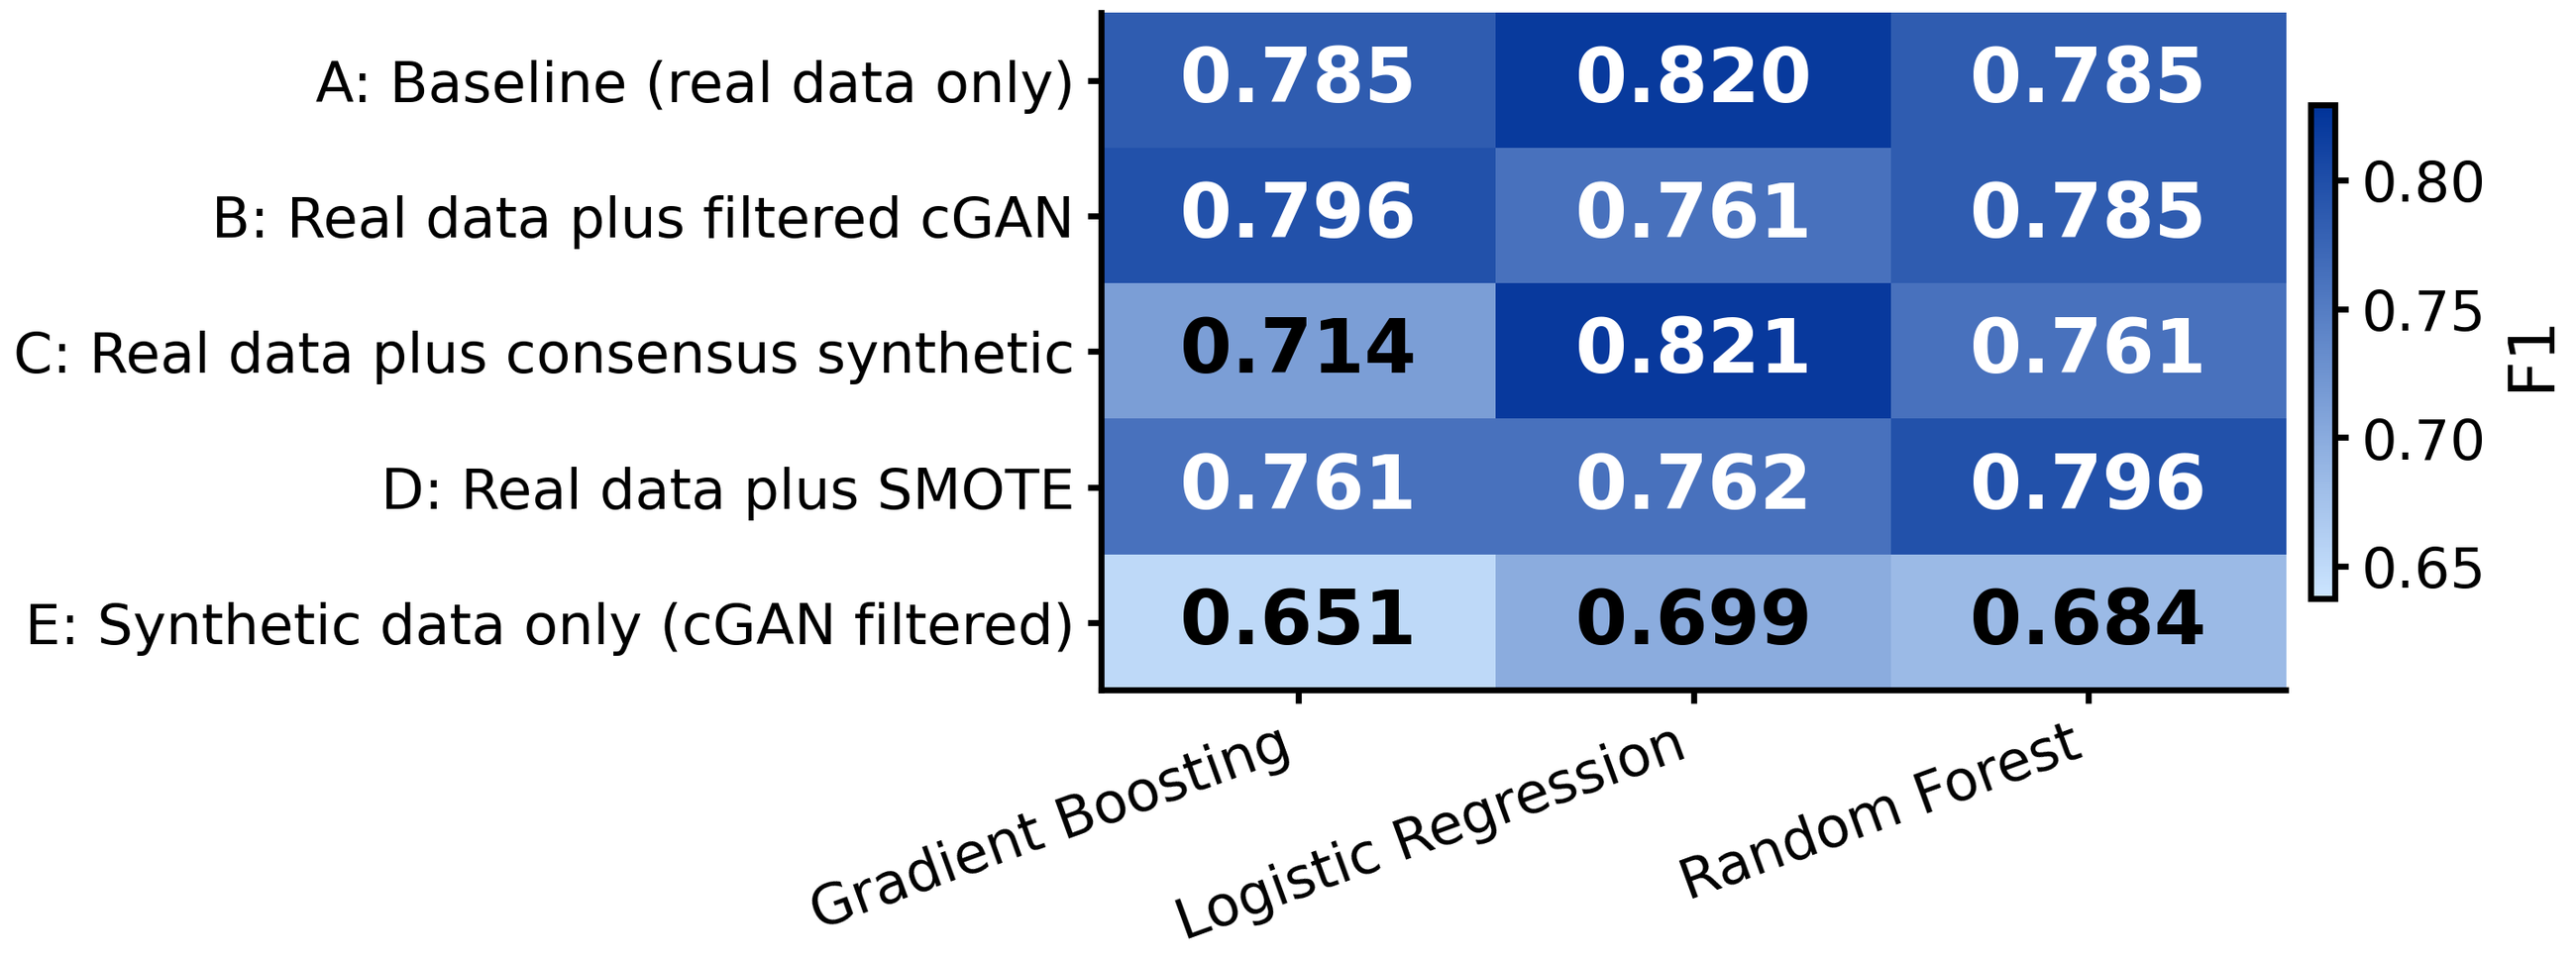
\includegraphics[width=\linewidth]{figS08_performance_heatmap.png}
  \caption{F1-score heatmap across training scenarios, N\_Days excluded from classifier input; darker shading indicates higher F1. Logistic Regression under Scenario~C achieves the highest F1 at 0.821. Under Scenario~C, Random Forest falls to 0.761 and Gradient Boosting to 0.714 while Logistic Regression is essentially unchanged (0.820 to 0.821), showing that consensus augmentation does not move all classifiers in the same direction.}
  \label{figS:heatmap}
\end{figure}

Figs.~\ref{figS:modelcomp} and~\ref{figS:allmetrics} present the same results grouped two further ways, the first by metric across all five scenarios and the second as metric trajectories per classifier. Both make the flatness of the comparison plain. Scenario~E, trained on synthetic data alone, is the only condition that separates clearly from the rest, and it does so downwards for Gradient Boosting while remaining competitive for Random Forest and Logistic Regression.

\begin{figure}[!tb]
  \centering
  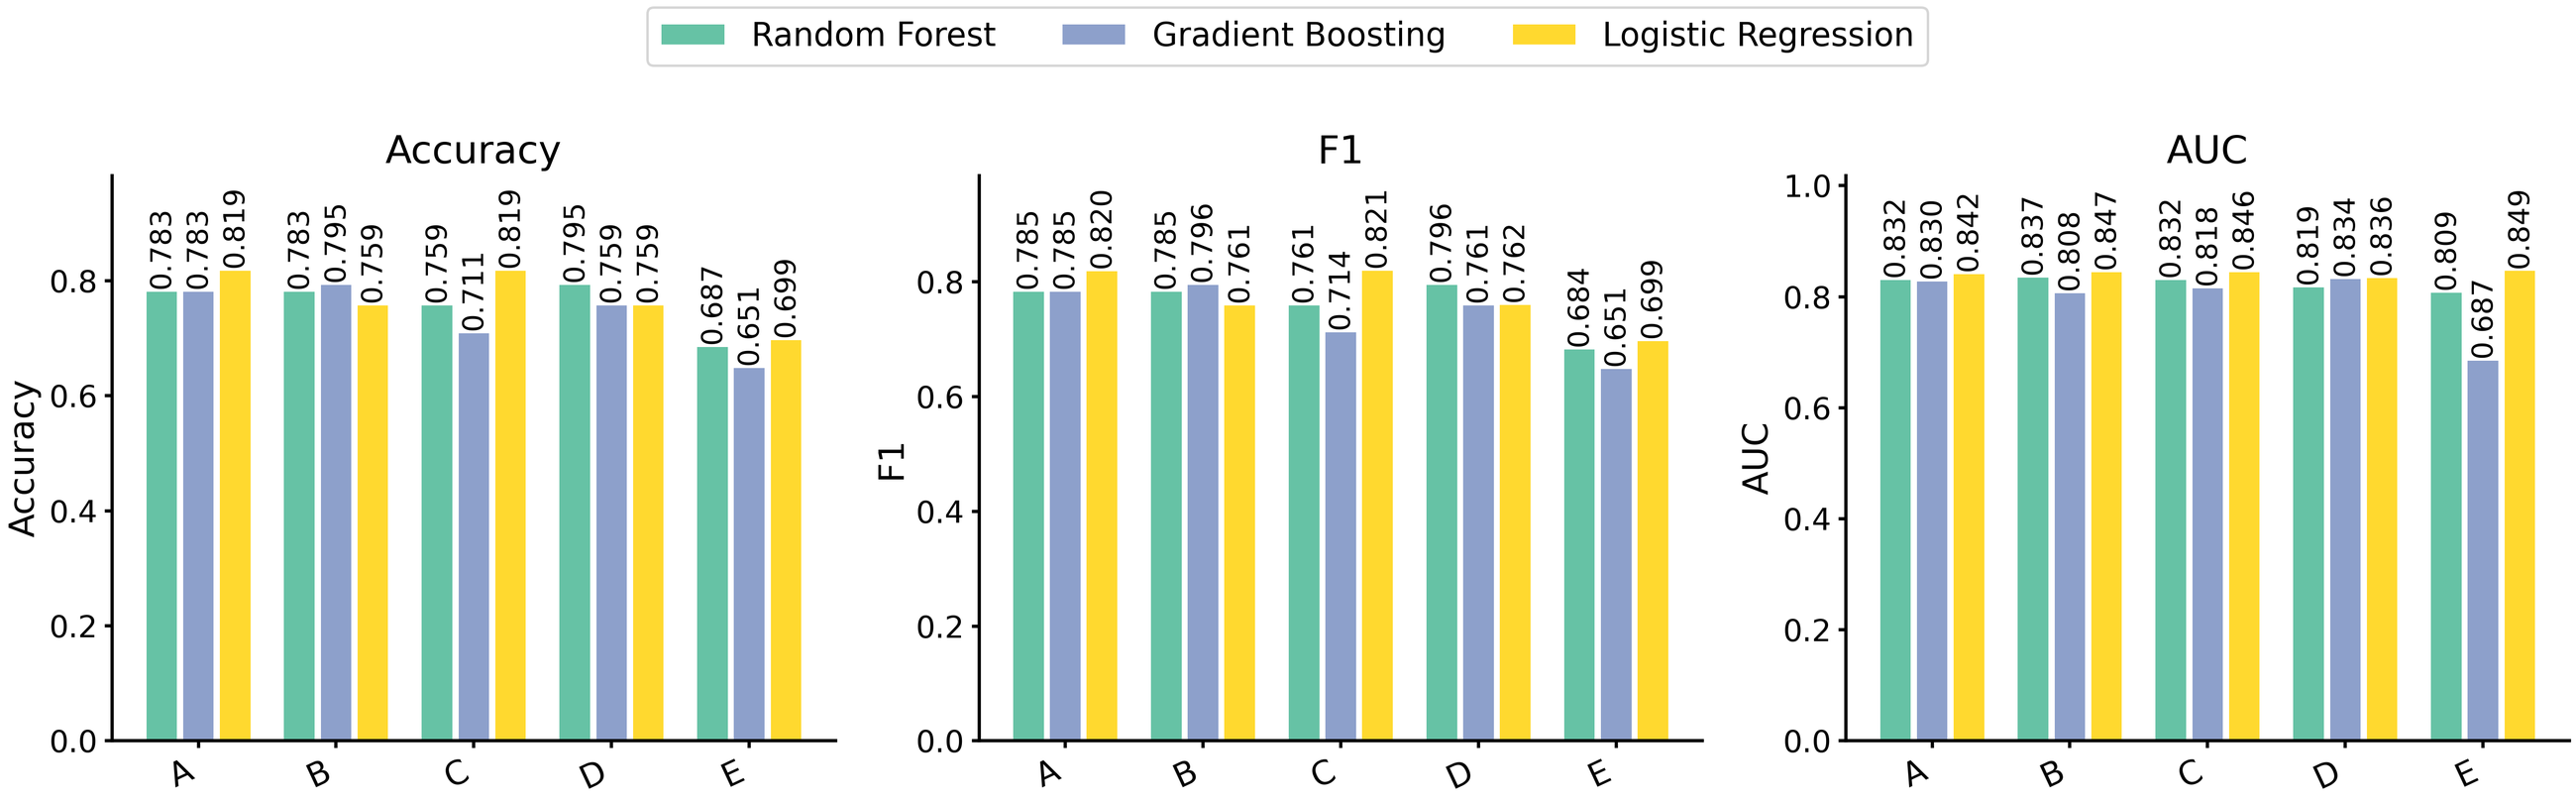
\includegraphics[width=\linewidth]{figS09_model_comparison.png}
  \caption{Grouped comparison of accuracy, F1 and AUC across all training scenarios and classifiers. No augmentation scenario uniformly outperforms the real-data baseline.}
  \label{figS:modelcomp}
\end{figure}

The grouped view in Fig.~\ref{figS:modelcomp} holds accuracy, F1 and AUC side by side so the three metrics can be compared within a scenario. The trajectory view that follows takes the opposite cut, following each metric across scenarios for a single classifier at a time.

\begin{figure}[!tb]
  \centering
  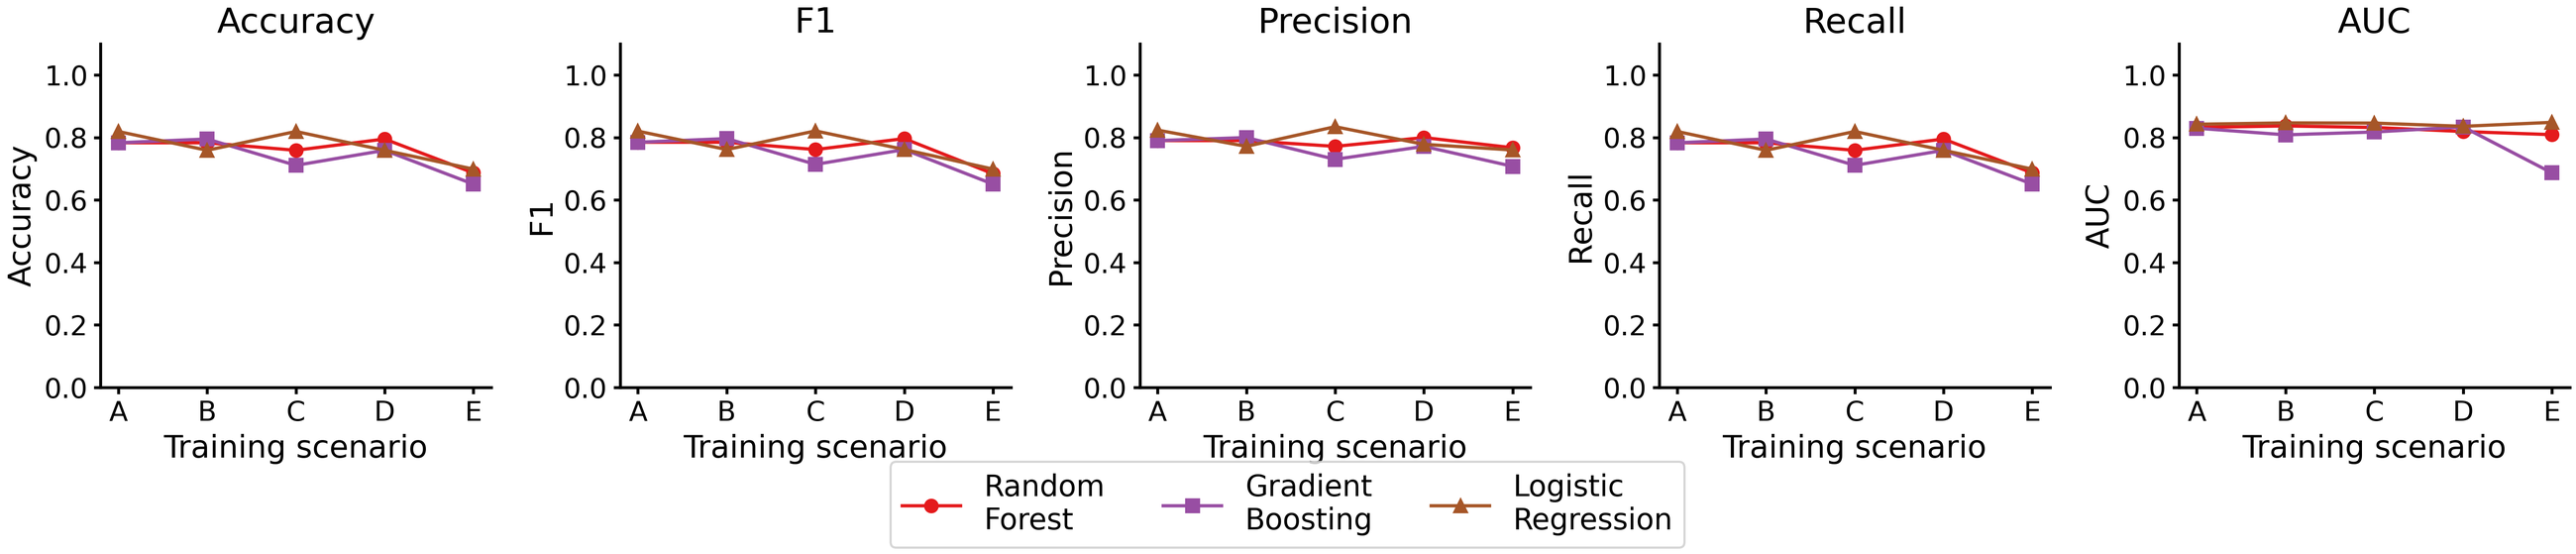
\includegraphics[width=\linewidth]{figS10_all_metrics.png}
  \caption{All five evaluation metrics across training scenarios for each classifier, N\_Days excluded from classifier input. Trajectories are flat or slightly declining from Scenario~A through Scenarios~B and~C, with Scenario~D (SMOTE) producing a modest accuracy gain for Random Forest only (0.783 to 0.795); Gradient Boosting and Logistic Regression both decline under Scenario~D.}
  \label{figS:allmetrics}
\end{figure}

% ===============================================================
\section{Competing Risks: Death Versus Transplant}
\label{sec:competingrisks}

The survival-modelling framing in Section~IV of the main paper (Cox proportional hazards, Random Survival Forest) treats death as the event of interest and censors at transplantation, alongside patients alive at data cutoff. This is a cause-specific hazard for death, a standard and defensible choice when death is the endpoint of interest, but it assumes transplant timing carries no information about death risk beyond what the covariates capture, an assumption worth checking rather than asserting, since transplant priority is itself driven by disease severity.

Of the 276 complete-case patients, 111 (40.2\%) died, 18 (6.5\%) received a transplant, and 147 (53.3\%) were censored alive at data cutoff. Fig.~\ref{figS:competingrisks} plots the non-parametric Aalen-Johansen cumulative incidence function for each competing event, which does not require the non-informative-censoring assumption the Cox/RSF analysis makes. Death dominates throughout follow-up: cumulative incidence reaches 64.2\% by the end of the observed follow-up window against 8.7\% for transplant, and the transplant curve stays near zero for the first roughly 500 days before rising gradually. Given how small the competing-event share is relative to the event of interest, censoring at transplant is unlikely to materially bias the cause-specific hazard estimates reported in the main paper, but a full competing-risks regression (e.g.\ a Fine-Gray subdistribution hazard model) would be needed to state that quantitatively rather than qualitatively; no Python package used in this pipeline currently implements one; \texttt{lifelines} provides the Aalen-Johansen estimator used here but not Fine-Gray regression.

\begin{figure}[!tb]
  \centering
  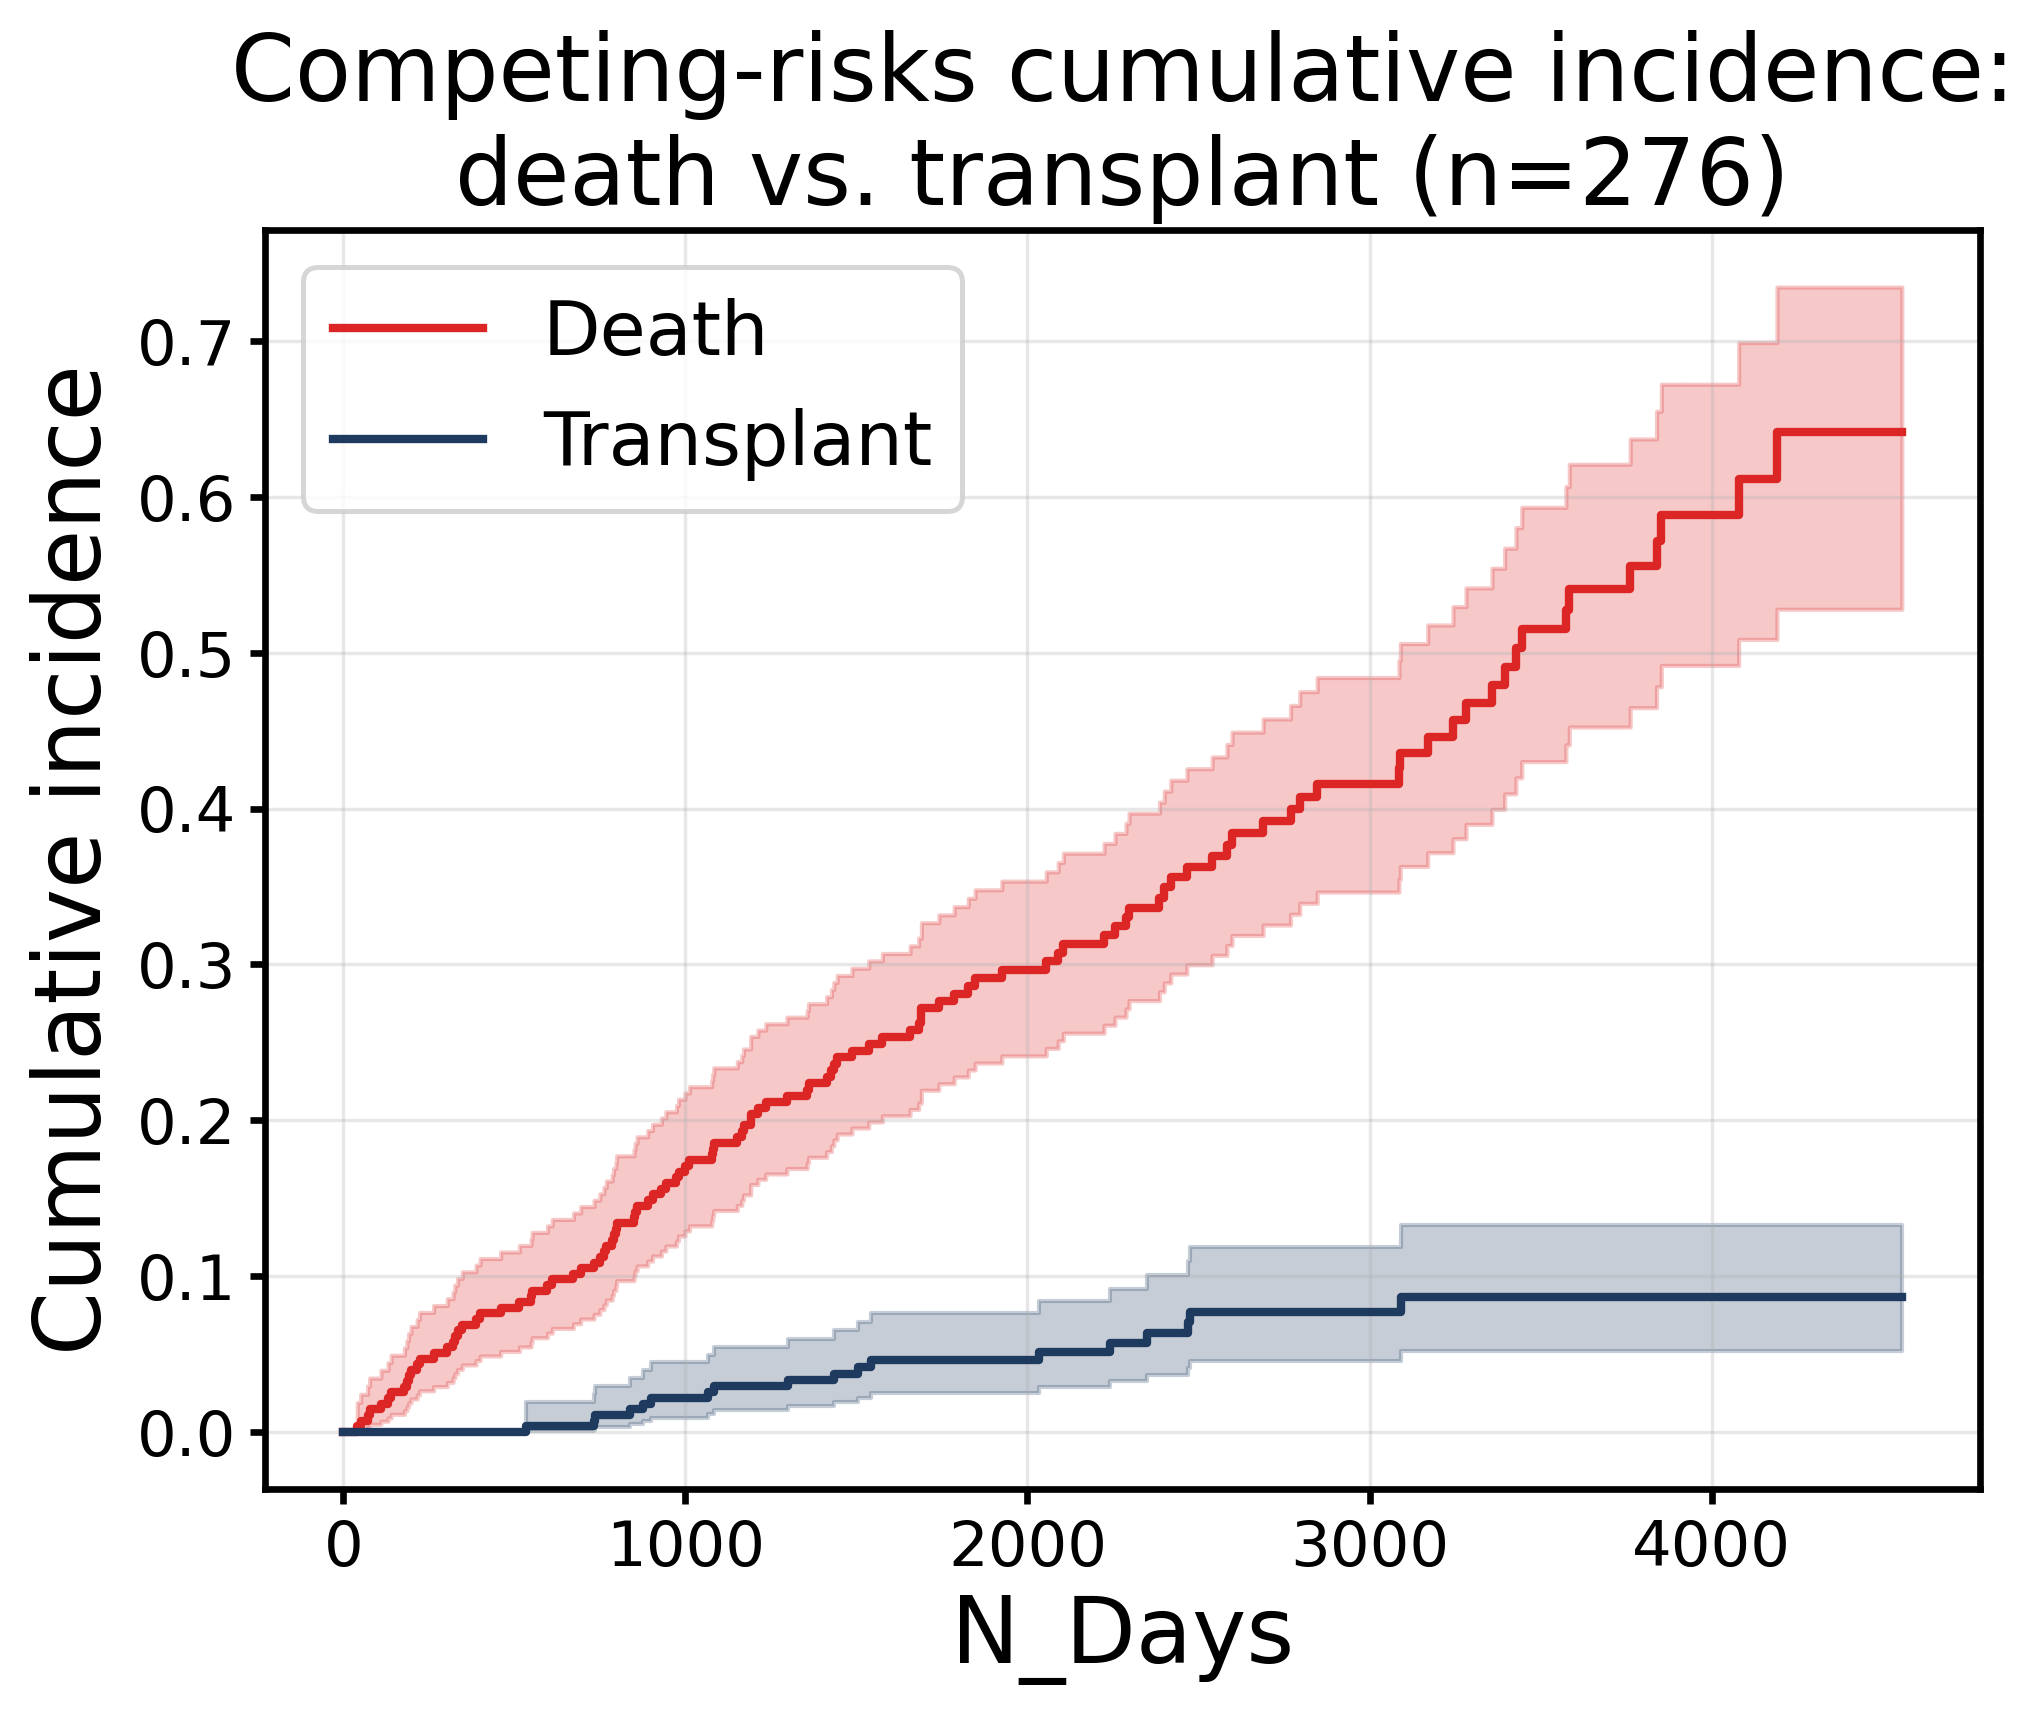
\includegraphics[width=0.68\linewidth]{figS11_competing_risks.png}
  \caption{Aalen-Johansen cumulative incidence of death and transplantation as competing events, computed on all 276 complete-case patients (shaded bands are 95\% confidence intervals). Death accounts for the large majority of observed events (64.2\% cumulative incidence by end of follow-up versus 8.7\% for transplant), supporting the cause-specific hazard treatment used in the main paper's survival framing while acknowledging it as a modelling choice rather than an assumption-free default.}
  \label{figS:competingrisks}
\end{figure}

% ===============================================================
\section{Kaplan-Meier Comparison Across Six Generators}
\label{sec:kmcomparison}

Section~IV of the main paper reports log-rank test statistics comparing each generator's synthetic (N\_Days, Status) distribution against the real training cohort, as a second check on whether FID predicts downstream utility. Fig.~\ref{figS:kmcomparison} gives the underlying Kaplan-Meier curves for all six generators.

\begin{figure*}[!t]
  \centering
  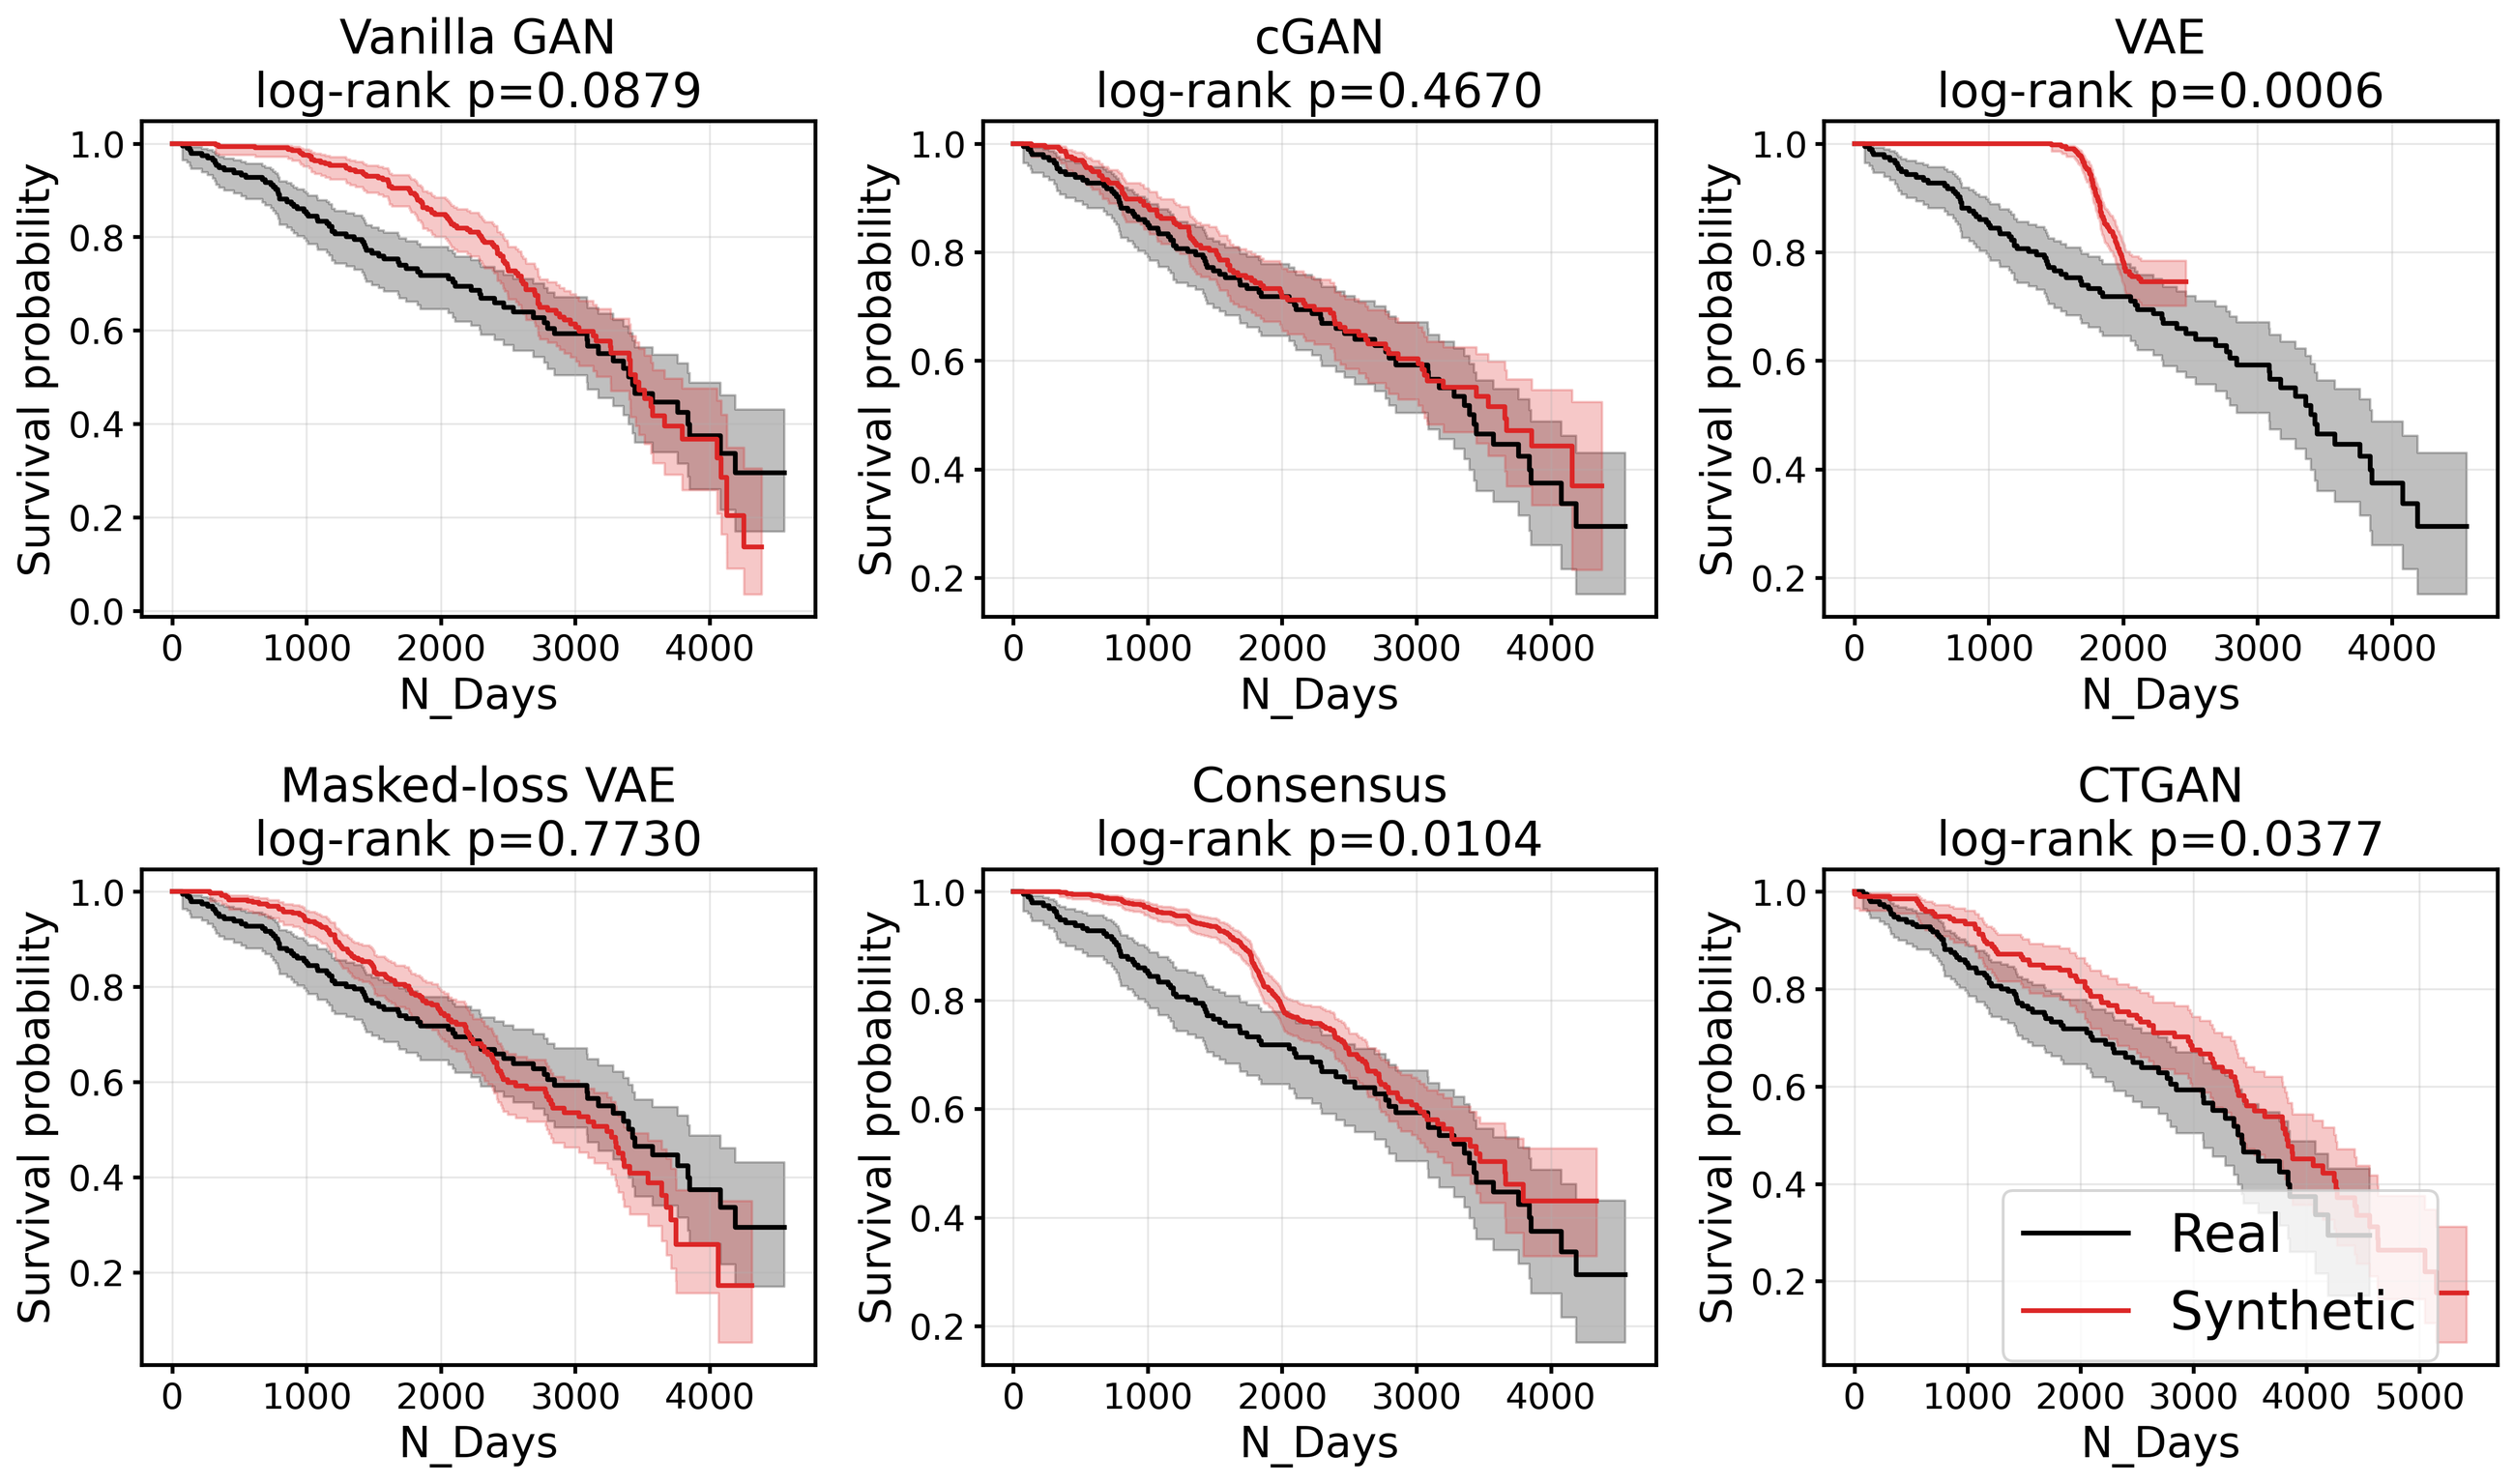
\includegraphics[width=0.98\textwidth]{figS12_km_comparison.png}
  \caption{Kaplan-Meier survival curves for each generator's synthetic (N\_Days, Status) pool (red) against the real training cohort (black), with log-rank test $p$-values. The masked-loss VAE and cGAN track the real curve closely; the VAE, CTGAN, and consensus diverge significantly, illustrating that FID does not isolate whether the joint time-to-event structure specifically is reproduced.}
  \label{figS:kmcomparison}
\end{figure*}

% ===============================================================
\section{Data and Code Availability}

The Mayo Clinic PBC dataset is publicly available from the UCI Machine Learning Repository as ``Cirrhosis Patient Survival Prediction'' (doi:~10.24432/C5R02G), \url{https://archive.ics.uci.edu/dataset/878/cirrhosis+patient+survival+prediction}. All code required to reproduce every number and figure in the main paper and in this document is available at \url{https://github.com/Michaeludousoro/liver-cirrhosis-synthetic-data}, including the generative models, the IQR and consensus filters, the evaluation pipeline, and the scripts that produce each supplementary table.

% ===============================================================
\section{Additional Supporting Figures}

The four figures below are referenced from earlier sections of this document (Extended Methodology and Extended Privacy Analyses) and are placed together here to keep this document's figure numbering stable as material is added.

\begin{figure*}[!t]
  \centering
  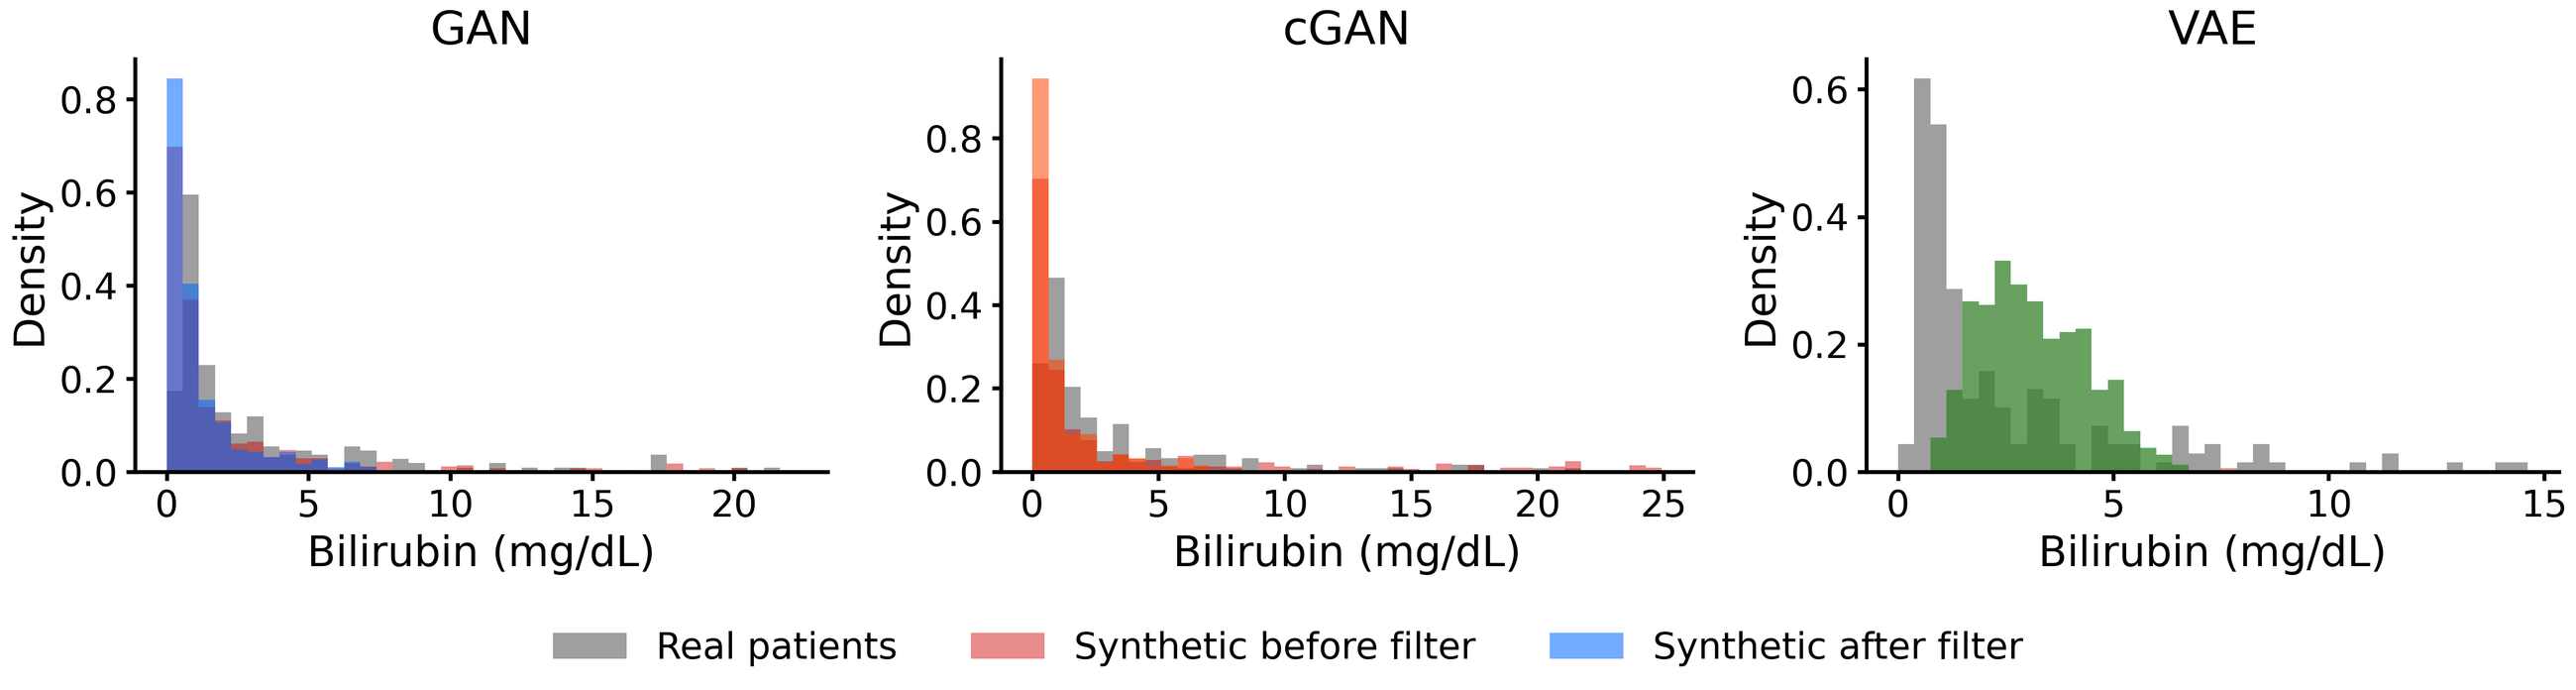
\includegraphics[width=0.98\textwidth]{figS13_iqr_filtering.png}
  \caption{Effect of IQR-based Tukey fence filtering on the Bilirubin distribution for all three generative models. Grey bars show real patient density. Pink bars show unfiltered synthetic distribution; coloured bars show the post-filter distribution. The GAN and cGAN produce records extending beyond 15~mg/dL that the filter removes. The VAE retains all generated records but produces a distribution shifted rightward relative to real patients.}
  \label{figS:iqr}
\end{figure*}

\begin{figure*}[!t]
  \centering
  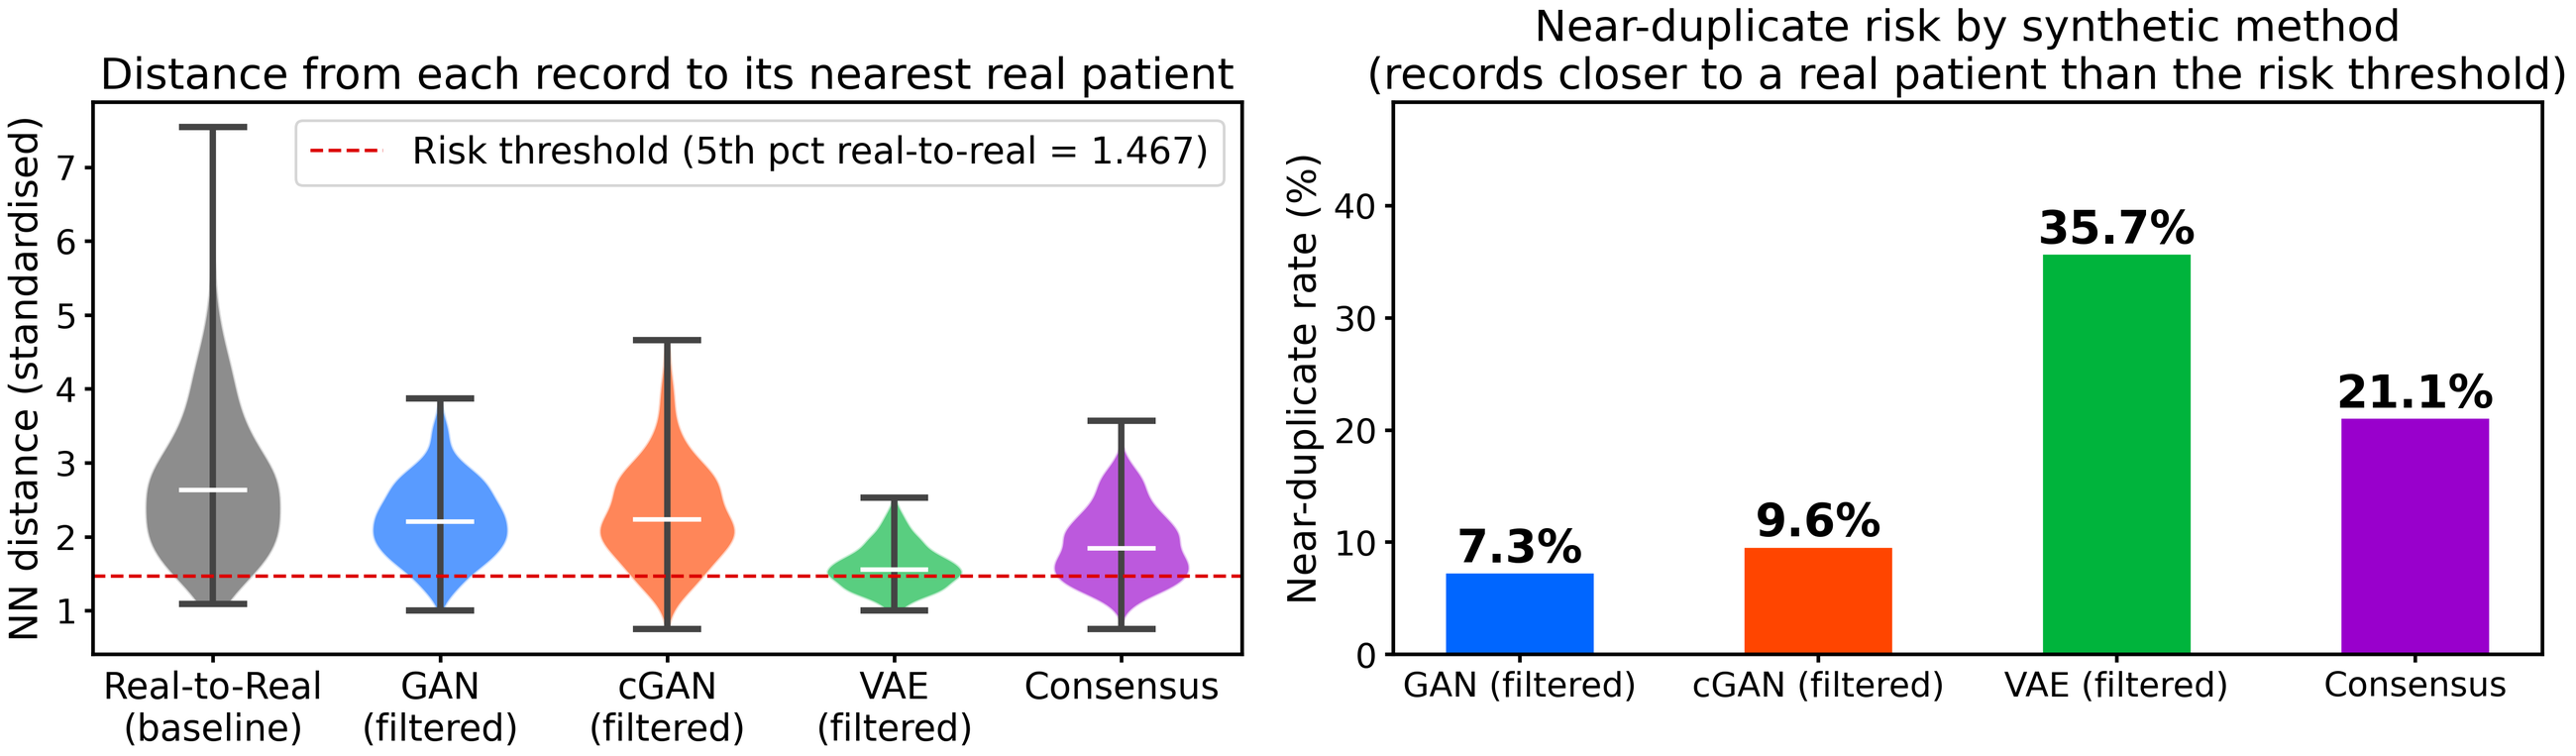
\includegraphics[width=0.98\textwidth]{figS14_privacy_risk_analysis.png}
  \caption{Privacy disclosure risk analysis using nearest-neighbour distances in standardised feature space. Left: violin plots of distances from each synthetic record to its closest real training patient. The red dashed line marks the risk threshold at the 5th percentile of real-to-real distances. GAN and cGAN distributions are centred above this threshold. Right: near-duplicate rates by method. GAN (7.3\%) and cGAN (9.6\%) present low privacy risk, VAE the highest at 35.7\%, and the equalised consensus set 21.1\%.}
  \label{figS:privacyrisk}
\end{figure*}

\begin{figure*}[!t]
  \centering
  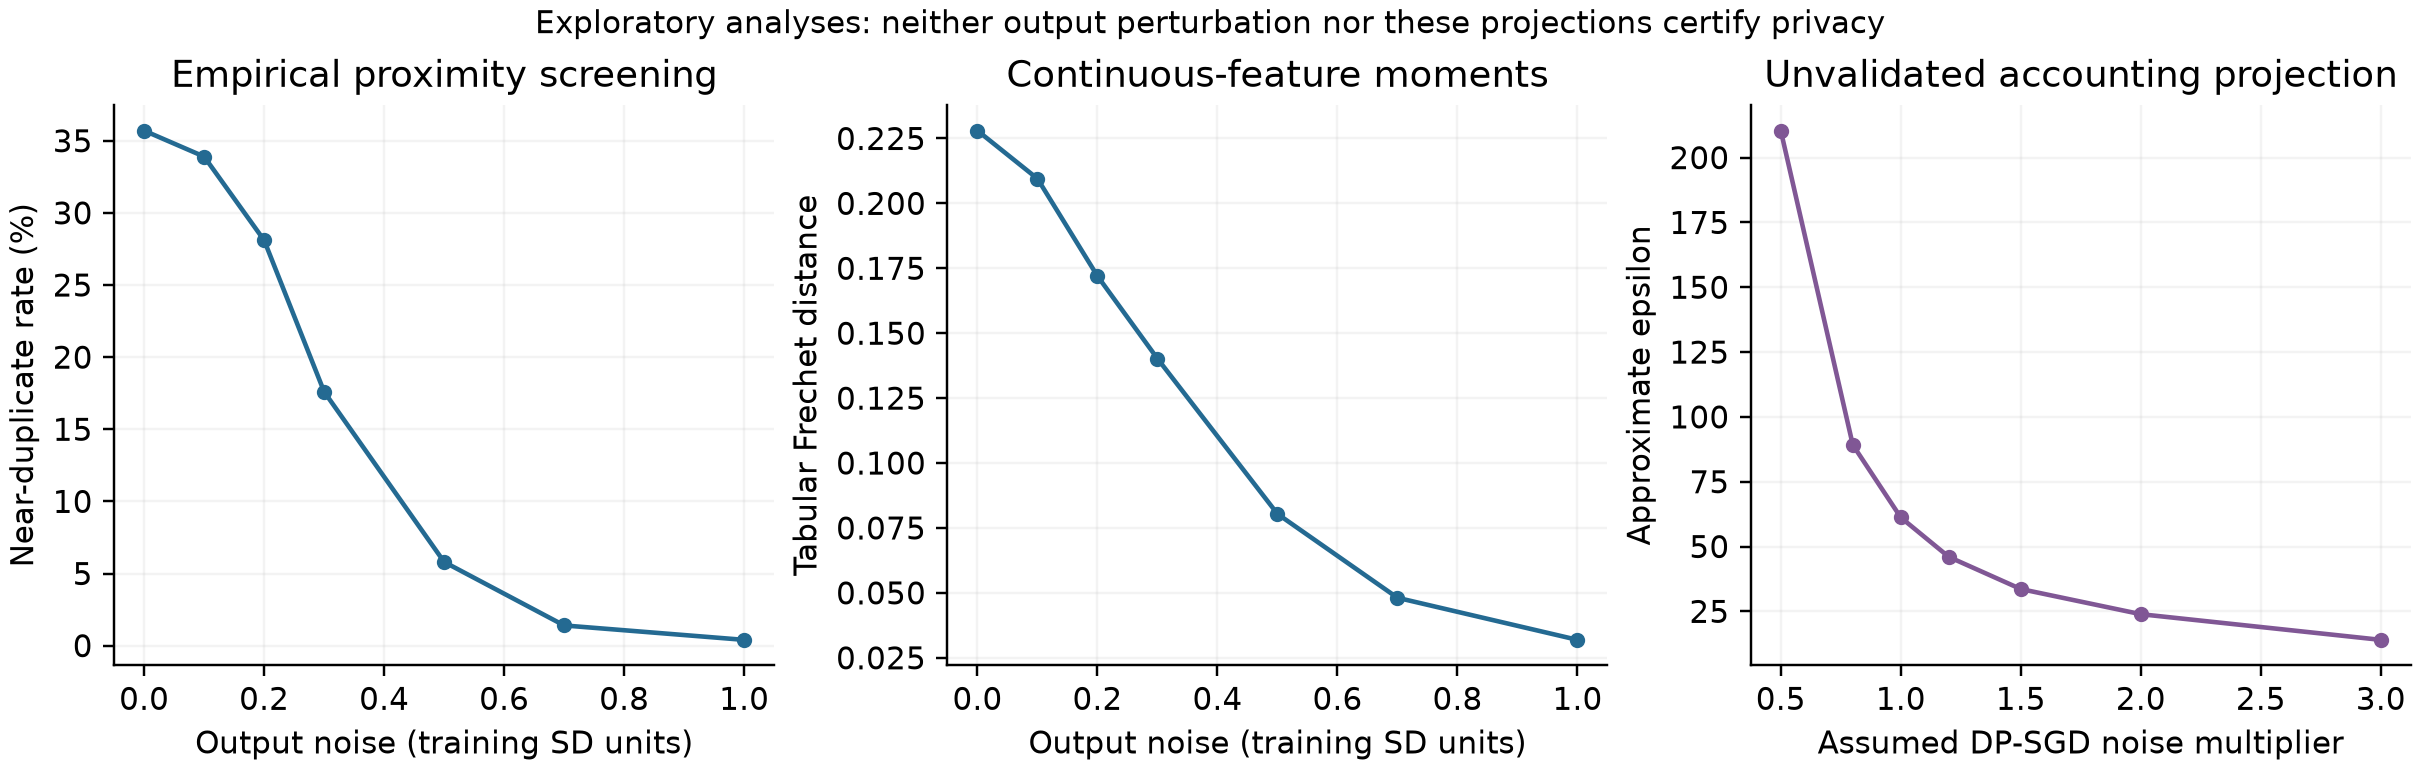
\includegraphics[width=0.98\textwidth]{figS15_privacy_enhancement.png}
  \caption{VAE privacy enhancement analysis. Left: near-duplicate rate versus Gaussian output noise $\sigma$ (in feature standard-deviation units); at $\sigma = 0.7$ the rate falls from 35.7\% to 1.4\%, crossing the 5\% near-duplicate target. Centre: tabular FID score versus $\sigma$; FID improves from 0.228 to 0.0481, below the equalised consensus benchmark of 0.0809. Right: estimated DP-SGD privacy budget $\varepsilon$ versus noise multiplier at $\delta = 10^{-5}$; $\varepsilon$ remains above 14 even at a multiplier of 3.0, confirming that formal differential privacy is not achievable at $n = 193$.}
  \label{figS:privacyenhance}
\end{figure*}

\begin{figure}[!tb]
  \centering
  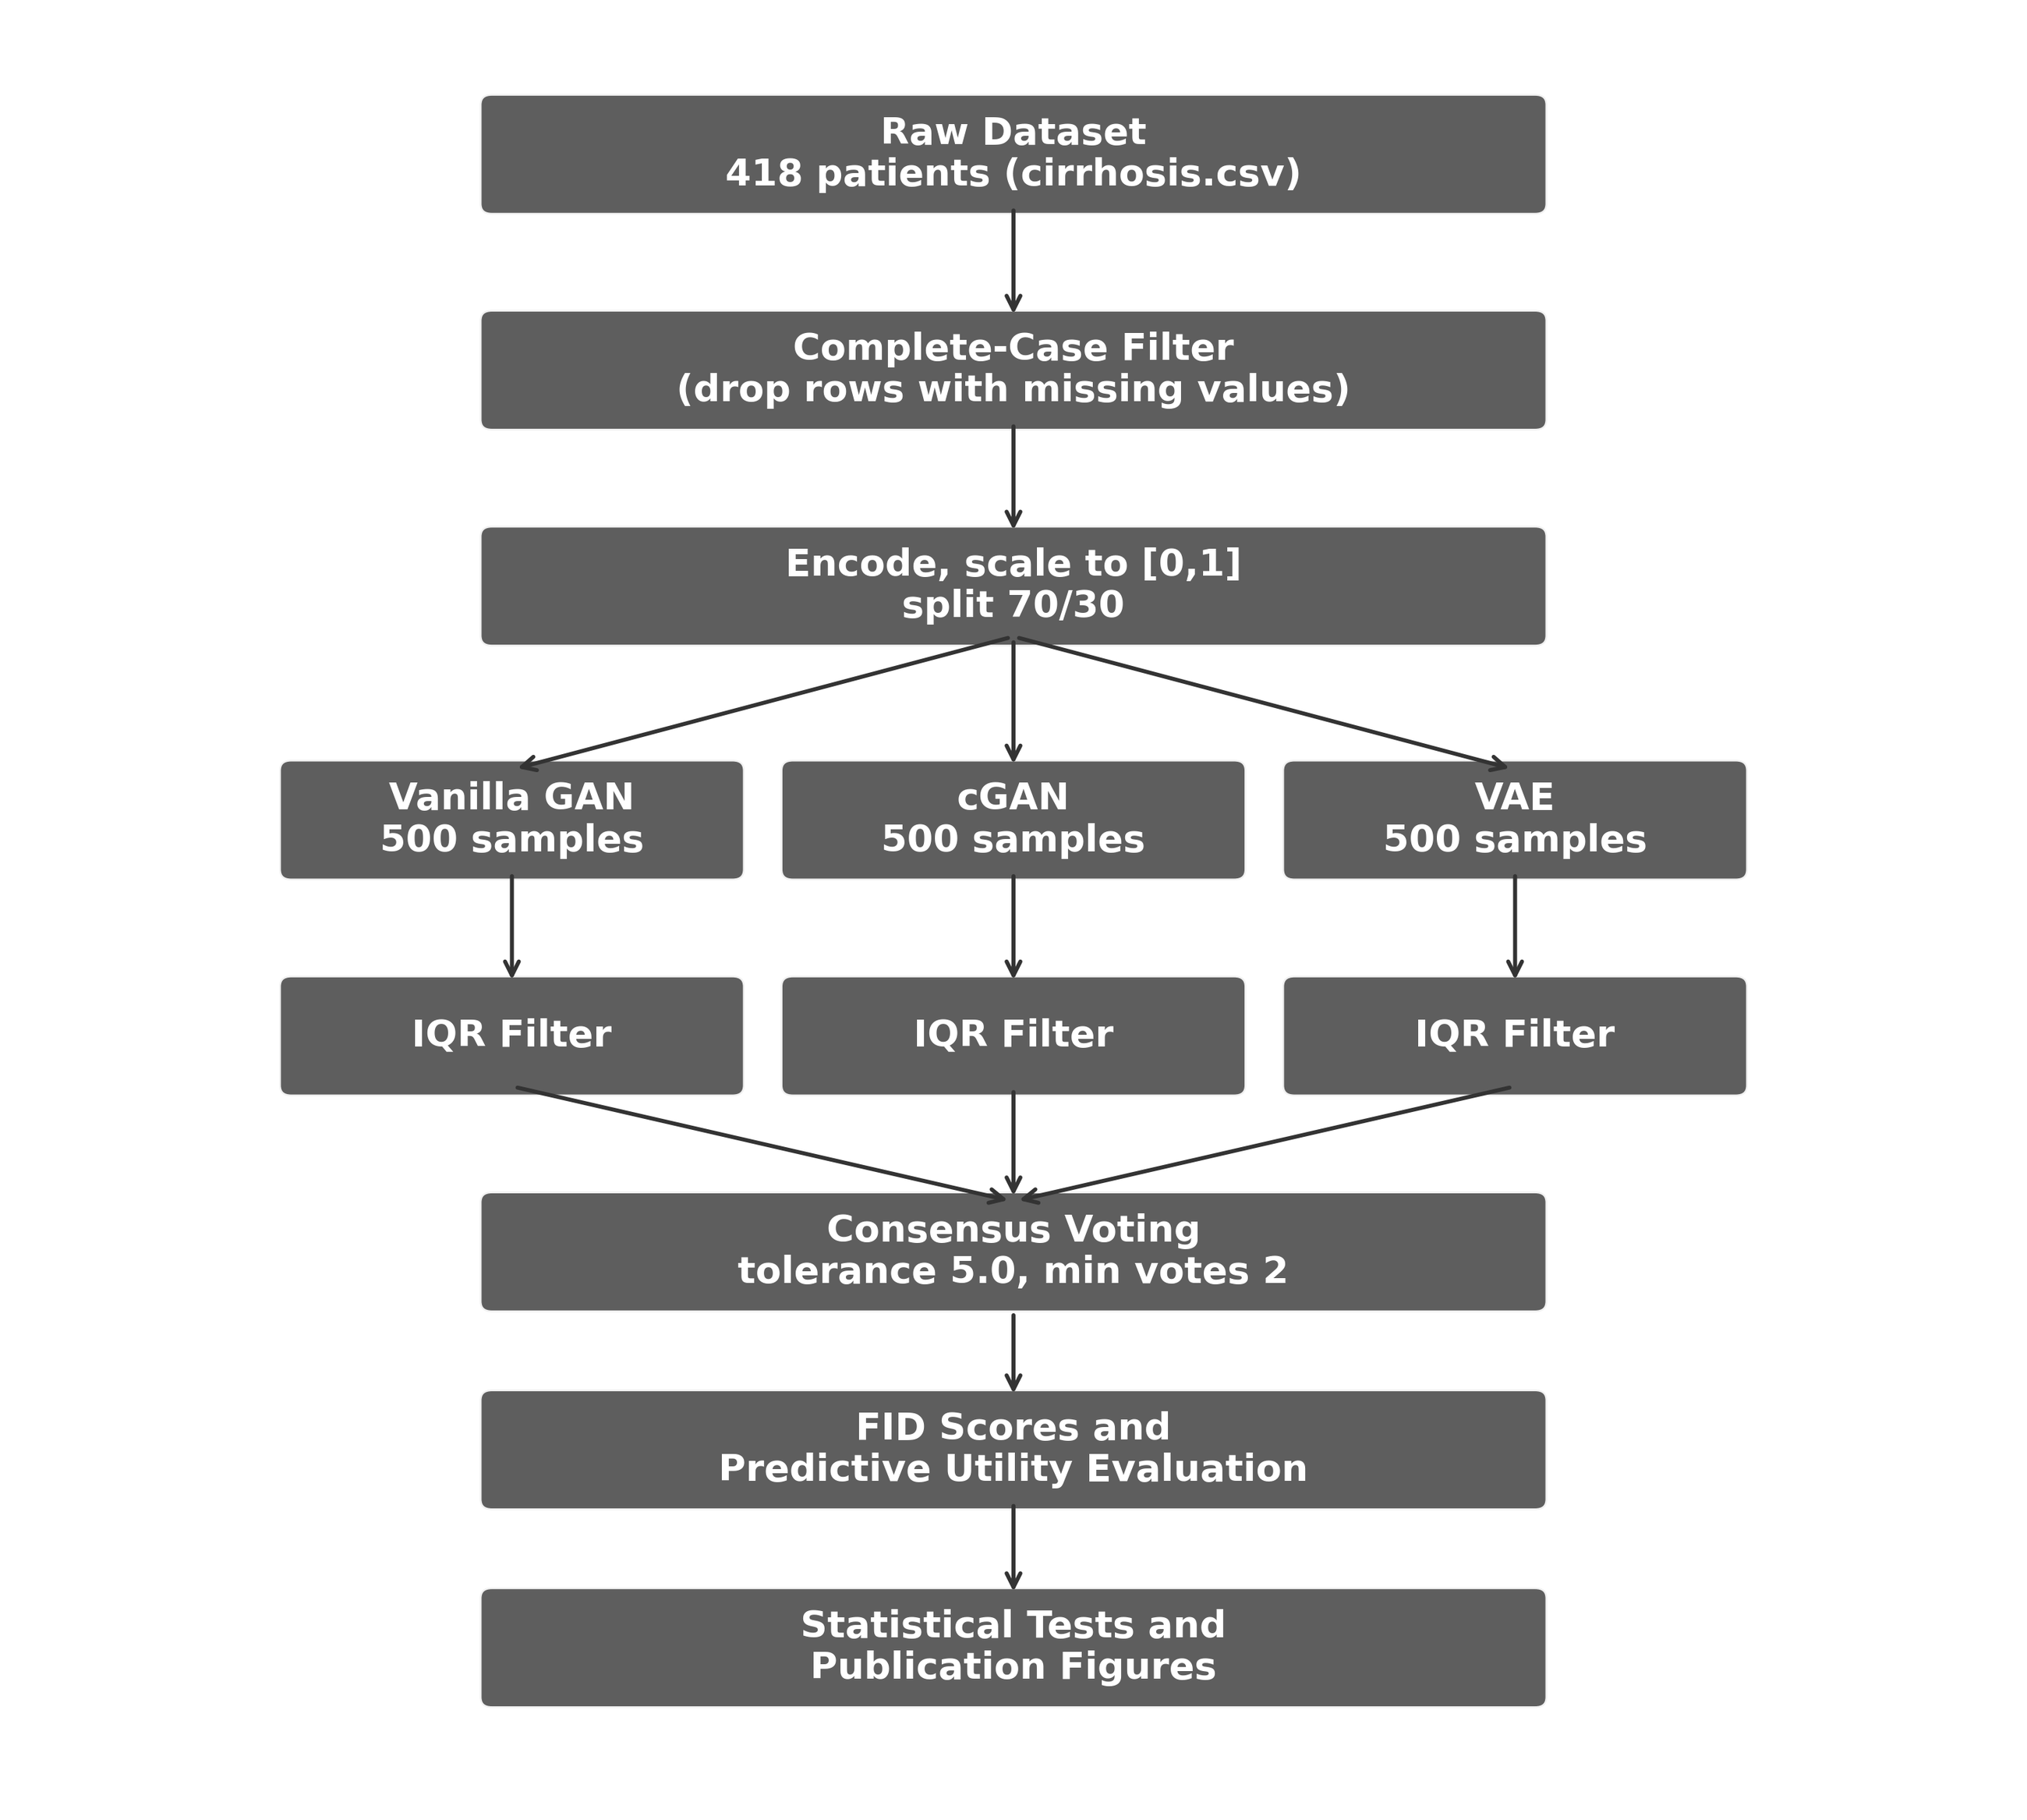
\includegraphics[width=\linewidth]{figS16_pipeline_flowchart.png}
  \caption{End-to-end synthetic data pipeline. The raw 418-patient dataset passes through a complete-case filter and a preprocessing stage before the 193-patient training set feeds three parallel generative models. Each model's 500 generated records pass through an IQR plausibility filter before all three filtered pools enter the consensus voting stage.}
  \label{figS:pipeline}
\end{figure}

\FloatBarrier
% ===============================================================
% References
% ===============================================================
\begin{thebibliography}{9}

\bibitem{mirza2014}
M. Mirza and S. Osindero, ``Conditional generative adversarial nets,'' \textit{arXiv}, Nov.~2014, doi:~10.48550/arxiv.1411.1784.

\bibitem{xu2019}
L. Xu, M. Skoularidou, A. Cuesta-Infante, and K. Veeramachaneni, ``Modeling tabular data using conditional GAN,'' in \textit{Proc. Adv. Neural Inf. Process. Syst. (NeurIPS)}, 2019, pp.~7335--7345.

\end{thebibliography}

\end{document}
